% Options for packages loaded elsewhere
\PassOptionsToPackage{unicode}{hyperref}
\PassOptionsToPackage{hyphens}{url}
\PassOptionsToPackage{dvipsnames,svgnames,x11names}{xcolor}
%
\documentclass[
  letterpaper,
  DIV=11,
  numbers=noendperiod]{scrreprt}

\usepackage{amsmath,amssymb}
\usepackage{lmodern}
\usepackage{iftex}
\ifPDFTeX
  \usepackage[T1]{fontenc}
  \usepackage[utf8]{inputenc}
  \usepackage{textcomp} % provide euro and other symbols
\else % if luatex or xetex
  \usepackage{unicode-math}
  \defaultfontfeatures{Scale=MatchLowercase}
  \defaultfontfeatures[\rmfamily]{Ligatures=TeX,Scale=1}
\fi
% Use upquote if available, for straight quotes in verbatim environments
\IfFileExists{upquote.sty}{\usepackage{upquote}}{}
\IfFileExists{microtype.sty}{% use microtype if available
  \usepackage[]{microtype}
  \UseMicrotypeSet[protrusion]{basicmath} % disable protrusion for tt fonts
}{}
\makeatletter
\@ifundefined{KOMAClassName}{% if non-KOMA class
  \IfFileExists{parskip.sty}{%
    \usepackage{parskip}
  }{% else
    \setlength{\parindent}{0pt}
    \setlength{\parskip}{6pt plus 2pt minus 1pt}}
}{% if KOMA class
  \KOMAoptions{parskip=half}}
\makeatother
\usepackage{xcolor}
\setlength{\emergencystretch}{3em} % prevent overfull lines
\setcounter{secnumdepth}{5}
% Make \paragraph and \subparagraph free-standing
\ifx\paragraph\undefined\else
  \let\oldparagraph\paragraph
  \renewcommand{\paragraph}[1]{\oldparagraph{#1}\mbox{}}
\fi
\ifx\subparagraph\undefined\else
  \let\oldsubparagraph\subparagraph
  \renewcommand{\subparagraph}[1]{\oldsubparagraph{#1}\mbox{}}
\fi

\usepackage{color}
\usepackage{fancyvrb}
\newcommand{\VerbBar}{|}
\newcommand{\VERB}{\Verb[commandchars=\\\{\}]}
\DefineVerbatimEnvironment{Highlighting}{Verbatim}{commandchars=\\\{\}}
% Add ',fontsize=\small' for more characters per line
\usepackage{framed}
\definecolor{shadecolor}{RGB}{241,243,245}
\newenvironment{Shaded}{\begin{snugshade}}{\end{snugshade}}
\newcommand{\AlertTok}[1]{\textcolor[rgb]{0.68,0.00,0.00}{#1}}
\newcommand{\AnnotationTok}[1]{\textcolor[rgb]{0.37,0.37,0.37}{#1}}
\newcommand{\AttributeTok}[1]{\textcolor[rgb]{0.40,0.45,0.13}{#1}}
\newcommand{\BaseNTok}[1]{\textcolor[rgb]{0.68,0.00,0.00}{#1}}
\newcommand{\BuiltInTok}[1]{\textcolor[rgb]{0.00,0.23,0.31}{#1}}
\newcommand{\CharTok}[1]{\textcolor[rgb]{0.13,0.47,0.30}{#1}}
\newcommand{\CommentTok}[1]{\textcolor[rgb]{0.37,0.37,0.37}{#1}}
\newcommand{\CommentVarTok}[1]{\textcolor[rgb]{0.37,0.37,0.37}{\textit{#1}}}
\newcommand{\ConstantTok}[1]{\textcolor[rgb]{0.56,0.35,0.01}{#1}}
\newcommand{\ControlFlowTok}[1]{\textcolor[rgb]{0.00,0.23,0.31}{#1}}
\newcommand{\DataTypeTok}[1]{\textcolor[rgb]{0.68,0.00,0.00}{#1}}
\newcommand{\DecValTok}[1]{\textcolor[rgb]{0.68,0.00,0.00}{#1}}
\newcommand{\DocumentationTok}[1]{\textcolor[rgb]{0.37,0.37,0.37}{\textit{#1}}}
\newcommand{\ErrorTok}[1]{\textcolor[rgb]{0.68,0.00,0.00}{#1}}
\newcommand{\ExtensionTok}[1]{\textcolor[rgb]{0.00,0.23,0.31}{#1}}
\newcommand{\FloatTok}[1]{\textcolor[rgb]{0.68,0.00,0.00}{#1}}
\newcommand{\FunctionTok}[1]{\textcolor[rgb]{0.28,0.35,0.67}{#1}}
\newcommand{\ImportTok}[1]{\textcolor[rgb]{0.00,0.46,0.62}{#1}}
\newcommand{\InformationTok}[1]{\textcolor[rgb]{0.37,0.37,0.37}{#1}}
\newcommand{\KeywordTok}[1]{\textcolor[rgb]{0.00,0.23,0.31}{#1}}
\newcommand{\NormalTok}[1]{\textcolor[rgb]{0.00,0.23,0.31}{#1}}
\newcommand{\OperatorTok}[1]{\textcolor[rgb]{0.37,0.37,0.37}{#1}}
\newcommand{\OtherTok}[1]{\textcolor[rgb]{0.00,0.23,0.31}{#1}}
\newcommand{\PreprocessorTok}[1]{\textcolor[rgb]{0.68,0.00,0.00}{#1}}
\newcommand{\RegionMarkerTok}[1]{\textcolor[rgb]{0.00,0.23,0.31}{#1}}
\newcommand{\SpecialCharTok}[1]{\textcolor[rgb]{0.37,0.37,0.37}{#1}}
\newcommand{\SpecialStringTok}[1]{\textcolor[rgb]{0.13,0.47,0.30}{#1}}
\newcommand{\StringTok}[1]{\textcolor[rgb]{0.13,0.47,0.30}{#1}}
\newcommand{\VariableTok}[1]{\textcolor[rgb]{0.07,0.07,0.07}{#1}}
\newcommand{\VerbatimStringTok}[1]{\textcolor[rgb]{0.13,0.47,0.30}{#1}}
\newcommand{\WarningTok}[1]{\textcolor[rgb]{0.37,0.37,0.37}{\textit{#1}}}

\providecommand{\tightlist}{%
  \setlength{\itemsep}{0pt}\setlength{\parskip}{0pt}}\usepackage{longtable,booktabs,array}
\usepackage{calc} % for calculating minipage widths
% Correct order of tables after \paragraph or \subparagraph
\usepackage{etoolbox}
\makeatletter
\patchcmd\longtable{\par}{\if@noskipsec\mbox{}\fi\par}{}{}
\makeatother
% Allow footnotes in longtable head/foot
\IfFileExists{footnotehyper.sty}{\usepackage{footnotehyper}}{\usepackage{footnote}}
\makesavenoteenv{longtable}
\usepackage{graphicx}
\makeatletter
\def\maxwidth{\ifdim\Gin@nat@width>\linewidth\linewidth\else\Gin@nat@width\fi}
\def\maxheight{\ifdim\Gin@nat@height>\textheight\textheight\else\Gin@nat@height\fi}
\makeatother
% Scale images if necessary, so that they will not overflow the page
% margins by default, and it is still possible to overwrite the defaults
% using explicit options in \includegraphics[width, height, ...]{}
\setkeys{Gin}{width=\maxwidth,height=\maxheight,keepaspectratio}
% Set default figure placement to htbp
\makeatletter
\def\fps@figure{htbp}
\makeatother
\newlength{\cslhangindent}
\setlength{\cslhangindent}{1.5em}
\newlength{\csllabelwidth}
\setlength{\csllabelwidth}{3em}
\newlength{\cslentryspacingunit} % times entry-spacing
\setlength{\cslentryspacingunit}{\parskip}
\newenvironment{CSLReferences}[2] % #1 hanging-ident, #2 entry spacing
 {% don't indent paragraphs
  \setlength{\parindent}{0pt}
  % turn on hanging indent if param 1 is 1
  \ifodd #1
  \let\oldpar\par
  \def\par{\hangindent=\cslhangindent\oldpar}
  \fi
  % set entry spacing
  \setlength{\parskip}{#2\cslentryspacingunit}
 }%
 {}
\usepackage{calc}
\newcommand{\CSLBlock}[1]{#1\hfill\break}
\newcommand{\CSLLeftMargin}[1]{\parbox[t]{\csllabelwidth}{#1}}
\newcommand{\CSLRightInline}[1]{\parbox[t]{\linewidth - \csllabelwidth}{#1}\break}
\newcommand{\CSLIndent}[1]{\hspace{\cslhangindent}#1}

\KOMAoption{captions}{tableheading}
\makeatletter
\@ifpackageloaded{tcolorbox}{}{\usepackage[many]{tcolorbox}}
\@ifpackageloaded{fontawesome5}{}{\usepackage{fontawesome5}}
\definecolor{quarto-callout-color}{HTML}{909090}
\definecolor{quarto-callout-note-color}{HTML}{0758E5}
\definecolor{quarto-callout-important-color}{HTML}{CC1914}
\definecolor{quarto-callout-warning-color}{HTML}{EB9113}
\definecolor{quarto-callout-tip-color}{HTML}{00A047}
\definecolor{quarto-callout-caution-color}{HTML}{FC5300}
\definecolor{quarto-callout-color-frame}{HTML}{acacac}
\definecolor{quarto-callout-note-color-frame}{HTML}{4582ec}
\definecolor{quarto-callout-important-color-frame}{HTML}{d9534f}
\definecolor{quarto-callout-warning-color-frame}{HTML}{f0ad4e}
\definecolor{quarto-callout-tip-color-frame}{HTML}{02b875}
\definecolor{quarto-callout-caution-color-frame}{HTML}{fd7e14}
\makeatother
\makeatletter
\makeatother
\makeatletter
\@ifpackageloaded{bookmark}{}{\usepackage{bookmark}}
\makeatother
\makeatletter
\@ifpackageloaded{caption}{}{\usepackage{caption}}
\AtBeginDocument{%
\ifdefined\contentsname
  \renewcommand*\contentsname{Table of contents}
\else
  \newcommand\contentsname{Table of contents}
\fi
\ifdefined\listfigurename
  \renewcommand*\listfigurename{List of Figures}
\else
  \newcommand\listfigurename{List of Figures}
\fi
\ifdefined\listtablename
  \renewcommand*\listtablename{List of Tables}
\else
  \newcommand\listtablename{List of Tables}
\fi
\ifdefined\figurename
  \renewcommand*\figurename{Figure}
\else
  \newcommand\figurename{Figure}
\fi
\ifdefined\tablename
  \renewcommand*\tablename{Table}
\else
  \newcommand\tablename{Table}
\fi
}
\@ifpackageloaded{float}{}{\usepackage{float}}
\floatstyle{ruled}
\@ifundefined{c@chapter}{\newfloat{codelisting}{h}{lop}}{\newfloat{codelisting}{h}{lop}[chapter]}
\floatname{codelisting}{Listing}
\newcommand*\listoflistings{\listof{codelisting}{List of Listings}}
\makeatother
\makeatletter
\@ifpackageloaded{caption}{}{\usepackage{caption}}
\@ifpackageloaded{subcaption}{}{\usepackage{subcaption}}
\makeatother
\makeatletter
\@ifpackageloaded{tcolorbox}{}{\usepackage[many]{tcolorbox}}
\makeatother
\makeatletter
\@ifundefined{shadecolor}{\definecolor{shadecolor}{rgb}{.97, .97, .97}}
\makeatother
\makeatletter
\makeatother
\ifLuaTeX
  \usepackage{selnolig}  % disable illegal ligatures
\fi
\IfFileExists{bookmark.sty}{\usepackage{bookmark}}{\usepackage{hyperref}}
\IfFileExists{xurl.sty}{\usepackage{xurl}}{} % add URL line breaks if available
\urlstyle{same} % disable monospaced font for URLs
\hypersetup{
  pdftitle={Computational Sociology (PGSP11583)},
  pdfauthor={Christopher Barrie},
  colorlinks=true,
  linkcolor={blue},
  filecolor={Maroon},
  citecolor={Blue},
  urlcolor={Blue},
  pdfcreator={LaTeX via pandoc}}

\title{Computational Sociology (PGSP11583)}
\author{Christopher Barrie}
\date{2022-08-23T00:00:00+03:00}

\begin{document}
\maketitle
\ifdefined\Shaded\renewenvironment{Shaded}{\begin{tcolorbox}[enhanced, borderline west={3pt}{0pt}{shadecolor}, boxrule=0pt, sharp corners, breakable, interior hidden, frame hidden]}{\end{tcolorbox}}\fi

\renewcommand*\contentsname{Table of contents}
{
\hypersetup{linkcolor=}
\setcounter{tocdepth}{2}
\tableofcontents
}
\bookmarksetup{startatroot}

\hypertarget{computational-sociology}{%
\chapter*{Computational Sociology}\label{computational-sociology}}
\addcontentsline{toc}{chapter}{Computational Sociology}

This is the course book we will be using for Computational Sociology
(PGSP11583).

\begin{Shaded}
\begin{Highlighting}[]
\FunctionTok{print}\NormalTok{(}\StringTok{"Computational Sociology"}\NormalTok{)}
\end{Highlighting}
\end{Shaded}

\begin{verbatim}
[1] "Computational Sociology"
\end{verbatim}

\begin{tcolorbox}[enhanced jigsaw, rightrule=.15mm, arc=.35mm, bottomrule=.15mm, colback=white, toprule=.15mm, breakable, left=2mm, colframe=quarto-callout-note-color-frame, leftrule=.75mm, opacityback=0]
\begin{minipage}[t]{5.5mm}
\textcolor{quarto-callout-note-color}{\faInfo}
\end{minipage}%
\begin{minipage}[t]{\textwidth - 5.5mm}
The book is a ``live'' document meaning I will be updating as we
progress together through the course.\end{minipage}%
\end{tcolorbox}

\hypertarget{license}{%
\section*{License}\label{license}}
\addcontentsline{toc}{section}{License}

This website is (and will always be) \textbf{free to use}, and is
licensed under the
\href{https://creativecommons.org/licenses/by-nc-nd/4.0/}{Creative
Commons Attribution-NonCommercial-NoDerivs 4.0} License.

\bookmarksetup{startatroot}

\hypertarget{course-overview}{%
\chapter*{Course Overview}\label{course-overview}}
\addcontentsline{toc}{chapter}{Course Overview}

This below gives details of course structure, outcomes, and assessment.

\hypertarget{learning-outcomes}{%
\section*{Learning outcomes}\label{learning-outcomes}}
\addcontentsline{toc}{section}{Learning outcomes}

This course will give students training in the use of various
computational methods in the social sciences. The course will prepare
students for dissertation work that uses digital trace data and/or
computational methods and will provide hands-on training in the use of
the R programming language and (some) Python.

The course will provide a venue for seminar discussion of examples using
these methods in the empirical social sciences as well as lectures on
the technical and/or statistical dimensions of their application.

\hypertarget{course-structure}{%
\section*{Course structure}\label{course-structure}}
\addcontentsline{toc}{section}{Course structure}

We will be using this online book for the ten-week course in
``Computational Sociology'' (PGSP11583). Each chapter contains the
readings for that week. The book also includes worksheets with example
code for how to conduct some of the text analysis techniques we discuss
each week.

Each week (with the partial exception of week 1), we will be discussing,
alternately, the substantive and technical dimensions of published
research in the empirical social sciences.

\hypertarget{course-theme}{%
\section*{Course theme}\label{course-theme}}
\addcontentsline{toc}{section}{Course theme}

In order to discipline the course, I have decided to focus on one theme
that is currently making headlines: the political consequences of social
media.

With this in mind, every two weeks we will be studying a different
phenomenon that has gained media attention: e.g., echo chambers,
misinformation, violence.

On alternate weeks, we will discuss how these phenomena have been
studied---using both computational and non-computational methods. In the
subsequent week, we will then go through some of the technical
dimensions of the methods used in the papers we study.

\hypertarget{course-pre-preparation}{%
\section*{Course pre-preparation}\label{course-pre-preparation}}
\addcontentsline{toc}{section}{Course pre-preparation}

\textbf{NOTE}: Before the lecture in Week 2, students should complete
two introductory R exercises.

\begin{enumerate}
\def\labelenumi{\arabic{enumi}.}
\item
  First, you should consult the introduction to file directories and
  Github \href{https://cjbarrie.github.io/CS-ED/intro.html}{here}. This
  is crucial to properly logging and saving the work you produce.
\item
  Second, you should consult the worksheet
  \href{https://cjbarrie.github.io/CS-ED/intro.html}{here}, which is an
  introduction to setting up and understanding the very basics of
  working in R. S
\item
  Third, Ugur Ozdemir has provided a more comprehensive introductory R
  course for the Research Training Centre at the University of Edinburgh
  and you can follow the instructions
  \href{https://research-training-centre.sps.ed.ac.uk/micro-methods/}{here}
  to access this.
\end{enumerate}

\hypertarget{reference-sources}{%
\section*{Reference sources}\label{reference-sources}}
\addcontentsline{toc}{section}{Reference sources}

There are two main reference texts that will be of use during this
course:

\begin{itemize}
\tightlist
\item
  Wickham, Hadley and Garrett Grolemund. R for Data Science:
  \url{https://r4ds.had.co.nz/}
\item
  Salganik, Matt. Bit by Bit: Social Research in the Digital Age:
  \url{https://www.bitbybitbook.com/}
\end{itemize}

\hypertarget{assessment}{%
\section*{Assessment}\label{assessment}}
\addcontentsline{toc}{section}{Assessment}

\hypertarget{fortnightly-worksheets}{%
\subsection*{Fortnightly worksheets}\label{fortnightly-worksheets}}
\addcontentsline{toc}{subsection}{Fortnightly worksheets}

Each fortnight, I will provide you with one worksheet that walks you
through how to implement a different computational technique. At the end
of these worksheets you will find a set of questions. \textbf{You should
buddy up with someone else in your class and go through these together.}

This is called ``pair programming'' and there's a reason we do this.
Firstly, coding can be an isolating and difficult thing---it's good to
bring a friend along for the ride! Secondly, if there's something you
don't know, maybe your buddy will. This saves you both time. Thirdly,
your buddy can check your code as you write it, and vice versa. Again,
this means both of you are working together to produce and check
something as you go along.

At the subsequent week's lecture, I will pick on a pair at random to
answer each one of that worksheet's questions (i.e., there is
\textasciitilde1/3 chance you're going to get picked each week). I will
ask you to walk us through your code. And remember: it's also fine if
you struggled and didn't get to the end! If you encountered an obstacle,
we can work through that together. All that matters to me is that you
\textbf{try}.

\hypertarget{fortnightly-flash-talks}{%
\subsection*{Fortnightly flash talks}\label{fortnightly-flash-talks}}
\addcontentsline{toc}{subsection}{Fortnightly flash talks}

On the weeks where you are not going to be tasked with a coding
assignment, you're not off the hook\ldots{} I will again be selecting a
pair at random (the same as your coding pair) to talk me through one of
the readings. I will pick a different pair for each reading (i.e.,
\textasciitilde{} 1/3 chance again).

Don't let this be cause of great anguish: I just want \textbf{two or
three minutes} where you lay out for me: 1) the research question; 2)
the data source; 3) the method; 4) the findings; 5) what you thought its
limitations were. The main portion of your flash talk should focus on
element 5).

For this last one, you will want to think about 1)-4); i.e., you will
want to think about whether it really answered the research question,
whether the data was appropriate for answering that question, whether
the method was appropriate for answering that question, and whether the
results show what the author claims they show. \textbf{I will provide
you wish an example flash talk at the first lecture.}

\hypertarget{final-assessment}{%
\subsection*{Final assessment}\label{final-assessment}}
\addcontentsline{toc}{subsection}{Final assessment}

Assessment takes the form of \textbf{one} summative assessment. This
will be a 4000 word essay on a subject of your choosing (with prior
approval by me). For this, you will be required to select from a range
of data sources I will provide. You may also suggest your own data
source.

You will be asked to: a) formulate a research question; b) use at least
one computational technique that we have studied; c) conduct an analysis
of the data source you have provided; d) write up the initial findings;
and e) outline potential extensions of your analysis.

You will then provide the code you used in reproducible (markdown)
format and will be assessed on both the substantive content of your
essay contribution (the social science part) as well as your
demonstrated competency in coding and text analysis (the computational
part).

\bookmarksetup{startatroot}

\hypertarget{managing-data-and-code}{%
\chapter*{Managing data and code}\label{managing-data-and-code}}
\addcontentsline{toc}{chapter}{Managing data and code}

\begin{tcolorbox}[enhanced jigsaw, rightrule=.15mm, arc=.35mm, bottomrule=.15mm, colback=white, toprule=.15mm, breakable, left=2mm, colframe=quarto-callout-note-color-frame, leftrule=.75mm, opacityback=0]
\begin{minipage}[t]{5.5mm}
\textcolor{quarto-callout-note-color}{\faInfo}
\end{minipage}%
\begin{minipage}[t]{\textwidth - 5.5mm}
The following introductory section is taken, in slightly adapted form,
from Jae Yeon Kim's ``Computational Thinking for Social Scientists.'' It
is reproduced here for ease of access. To consult the full book, go to
\url{https://jaeyk.github.io/comp_thinking_social_science/}.\end{minipage}%
\end{tcolorbox}

\hypertarget{the-command-line}{%
\section*{The Command Line}\label{the-command-line}}
\addcontentsline{toc}{section}{The Command Line}

What is the command line? The command line or ``terminal'' is what
you'll recognize from Hollywood portrayals of hackers and script
kids---a black screen containing single lines of code, sometimes
cascading down the page.

But you all have one on your computers.

On Windows computers, you'll find this under the name ``Command
Prompt.'' See this
\href{https://www.wikihow.com/Open-Terminal-in-Windows}{guide} on how to
open.

On Mac, this is called ``Terminal''. See this
\href{https://www.wikihow.com/Open-a-Terminal-Window-in-Mac}{guide}.
Some also prefer to use an application called ``iTerm 2'' but they both
essentially do the same thing.

\hypertarget{the-big-picture}{%
\subsection*{The Big Picture}\label{the-big-picture}}
\addcontentsline{toc}{subsection}{The Big Picture}

As William Shotts the author of
\href{http://linuxcommand.org/tlcl.php}{\emph{The Linux Command Line}}
put it:

\begin{quote}
graphical user interfaces make easy tasks easy, while command-line
interfaces make difficult tasks possible.
\end{quote}

\hypertarget{why-bother-using-the-command-line}{%
\subsection*{Why bother using the command
line?}\label{why-bother-using-the-command-line}}
\addcontentsline{toc}{subsection}{Why bother using the command line?}

Suppose that we want to create a plain text file that contains the word
``test.'' If we want to do this in the command line, you need to know
the following commands.

\begin{enumerate}
\def\labelenumi{\arabic{enumi}.}
\tightlist
\item
  \texttt{echo}: ``Write arguments to the standard output'' This is
  equivalent to using a text editor (e.g., nano, vim, emacs) and writing
  something.
\item
  \texttt{\textgreater{}\ test} Save the expression in a file named
  test.
\end{enumerate}

We can put these commands together like the following:

\begin{Shaded}
\begin{Highlighting}[]
\BuiltInTok{echo} \StringTok{"sth"} \OperatorTok{\textgreater{}}\NormalTok{ test }
\end{Highlighting}
\end{Shaded}

Don't worry if you are worried about memorizing these and more commands.
Memorization is a far less important aspect of learning programming. In
general, if you don't know what a command does, just type
\texttt{\textless{}command\ name\textgreater{}\ -\/-help.} You can do
\texttt{man\ \textless{}command\ name\textgreater{}} to obtain further
information. Here, \texttt{man} stands for manual. If you need more
user-friendly information, please consider using
\href{https://tldr.sh/}{\texttt{tldr}}.

Let's make this simple case complex by scaling up. Suppose we want to
make 100 duplicates of the \texttt{test} file. Below is the one-line
code that performs the task!

\begin{Shaded}
\begin{Highlighting}[]
\ControlFlowTok{for}\NormalTok{ i }\KeywordTok{in} \DataTypeTok{\{}\DecValTok{1}\DataTypeTok{..}\DecValTok{100}\DataTypeTok{\}}\KeywordTok{;} \ControlFlowTok{do} \FunctionTok{cp}\NormalTok{ test }\StringTok{"test\_}\VariableTok{$i}\StringTok{"}\KeywordTok{;} \ControlFlowTok{done}  
\end{Highlighting}
\end{Shaded}

Let me break down the seemingly complex workflow.

\begin{enumerate}
\def\labelenumi{\arabic{enumi}.}
\item
  \texttt{for\ i\ in\ \{1..100\}.} This is a for loop. The numbers
  1..100 inside the curly braces \texttt{\{\}} indicates the range of
  integers from 1 to 100. In R, this is equivalent to for (i in 1:100)
  \{\}\\
\item
  \texttt{;} is used to use multiple commands without making line
  breaks. ; works in the same way in R.
\item
  \texttt{\$var} returns the value associated with a variable. Type
  \texttt{name=\textless{}Your\ name\textgreater{}}. Then, type
  \texttt{echo\ \$name.} You should see your name printed. Variable
  assignment is one of the most basic things you'll learn in any
  programming. In R, we do this by using -\textgreater{}
\end{enumerate}

If you have zero experience in programming, I might have provided too
many concepts too early, like variable assignment and for loop. However,
you don't need to worry about them at this point. We will cover them in
the next chapter.

I will give you one more example to illustrate how powerful the command
line is. Suppose we want to find which file contains the character
``COVID.'' This is equivalent to finding a needle in a haystack. It's a
daunting task for humans, but not for computers. Commands are verbs. So,
to express this problem in a language that computers could understand,
let's first find what command we should use. Often, a simple Google or
\href{https://stackoverflow.com/}{Stack Overflow} search leads to an
answer.

In this case, \texttt{grep} is the answer (there's also grep in R). This
command finds PATTERNS in each FILE. What follows - are options (called
flags): \texttt{r} (recursive), \texttt{n} (line number), \texttt{w}
(match only whole words), \texttt{e} (use patterns for matching).
\texttt{rnw} are for output control and \texttt{e} is for pattern
selection.

So, to perform the task above, you just need one-line code:
\texttt{grep\ -r\ -n\ -w\ -e\ "COVID\textquotesingle{}\textquotesingle{}}

\textbf{Quick reminders} - \texttt{grep}: command - \texttt{-rnw\ -e}:
flags - \texttt{COVID}: argument (usually file or file paths)

Let's remove (=\texttt{rm}) all the duplicate files and the original
file. \texttt{*} (any number of characters) is a wildcard (if you want
to identify a single number of characters, use \texttt{?}). It finds
every file whose name starts with \texttt{test\_}.

\begin{Shaded}
\begin{Highlighting}[]
\FunctionTok{rm}\NormalTok{ test\_}\PreprocessorTok{*}\NormalTok{ test }
\end{Highlighting}
\end{Shaded}

Enough with demonstrations. What is this black magic? Can you do the
same thing using a graphical interface? Which method is more efficient?
I hope that my demonstrations give you enough sense of why learning the
command line could be incredibly useful. In my experience, mastering the
command line helps automate your research process from end to end. For
instance, you don't need to write files from a website using your web
browser. Instead, you can run the \texttt{wget} command in the terminal.
Better yet, you don't even need to run the command for the second time.
You can write a Shell script (\texttt{*.sh}) that automates downloading,
moving, and sorting multiple files.

\hypertarget{unix-shell}{%
\subsection*{UNIX Shell}\label{unix-shell}}
\addcontentsline{toc}{subsection}{UNIX Shell}

The other thing you might have noticed is that there are many overlaps
between the commands and base R functions (R functions that can be used
without installing additional packages). This connection is not
coincident. UNIX preceded and influenced many programming languages,
including R.

The following materials on UNIX and Shell are adapted from {[}the
software
carpentry{]}(https://bids.GitHub.io/2015-06-04-berkeley/shell/00-intro.html.

\hypertarget{unix}{%
\subsubsection*{Unix}\label{unix}}
\addcontentsline{toc}{subsubsection}{Unix}

UNIX is an \textbf{operating system + a set of tools (utilities)}. It
was developed by AT \& T employees at Bell Labs (1969-1971). From Mac OS
X to Linux, many of the current operation systems are some versions of
UNIX. Command-line INTERFACE is a way to communicate with your OS by
typing, not pointing, and clicking.

For this reason, if you're using Mac OS, then you don't need to do
anything else to experience UNIX. You're already all set.

If you're using Windows, you need to install either GitBash (a good
option if you only use Bash for Git and GitHub) or Windows Subsystem
(highly recommended if your use case goes beyond Git and GitHub). For
more information, see
\href{https://github.com/cjbarrie/CS-ED/blob/main/other/setup.md}{this
installation guideline}. If you're a Windows user and don't use Windows
10, I recommend installing
\href{https://www.virtualbox.org/}{VirtualBox}.

UNIX is old, but it is still mainstream, and it will be. Moreover,
\href{https://en.wikipedia.org/wiki/Unix_philosophy}{the UNIX
philosophy} (``Do One Thing And Do It Well'')---minimalist, modular
software development---is highly and widely influential.

\hypertarget{kernel}{%
\subsubsection*{Kernel}\label{kernel}}
\addcontentsline{toc}{subsubsection}{Kernel}

The kernel of UNIX is the hub of the operating system: it allocates time
and memory to programs. It handles the
\href{http://users.ox.ac.uk/~martinw/unix/chap3.html}{filestore} (e.g.,
files and directories) and communications in response to system calls.

\hypertarget{shell}{%
\subsubsection*{Shell}\label{shell}}
\addcontentsline{toc}{subsubsection}{Shell}

The shell is an interactive program that provides an interface between
the user and the kernel. The shell interprets commands entered by the
user or supplied by a Shell script and passes them to the kernel for
execution.

\hypertarget{human-computer-interfaces}{%
\subsubsection*{Human-Computer
interfaces}\label{human-computer-interfaces}}
\addcontentsline{toc}{subsubsection}{Human-Computer interfaces}

At a high level, computers do four things:

\begin{itemize}
\tightlist
\item
  run programs
\item
  store data
\item
  communicate with each other
\item
  interact with us (through either CLI or GUI)
\end{itemize}

\hypertarget{the-command-line-1}{%
\subsubsection*{The Command Line}\label{the-command-line-1}}
\addcontentsline{toc}{subsubsection}{The Command Line}

This kind of interface is called a \textbf{command-line interface}, or
CLI, to distinguish it from the \textbf{graphical user interface}, or
GUI, that most people now use.

The heart of a CLI is a \textbf{read-evaluate-print loop}, or REPL: when
the user types a command and then presses the enter (or return) key, the
computer reads it, executes it, and prints its output. The user then
types another command, and so on until the user logs off.

If you're using RStudio, you can use terminal inside RStudio (next to
the ``Console''). (For instance, type Alt + Shift + M)

\hypertarget{the-shell}{%
\subsubsection*{The Shell}\label{the-shell}}
\addcontentsline{toc}{subsubsection}{The Shell}

This description makes it sound as though the user sends commands
directly to the computer and sends the output directly to the user. In
fact, there is usually a program in between called a \textbf{command
shell}.

\begin{figure}

{\centering 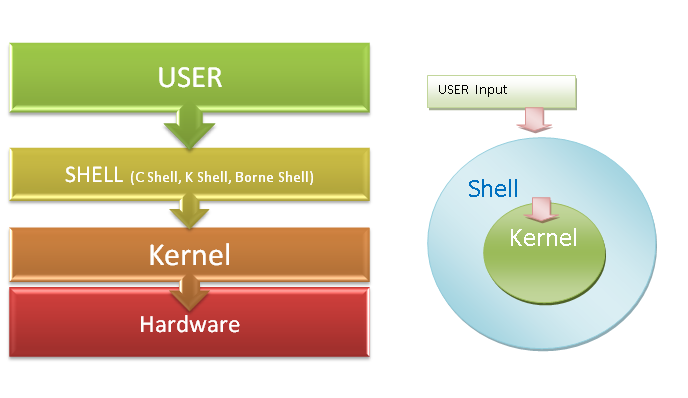
\includegraphics{./images/shell.png}

}

\caption{Source: Prashant Lakhera}

\end{figure}

What the user types go into the shell; it figures out what commands to
run and orders the computer to execute them.

Note, the shell is called \emph{the shell}: it encloses the operating
system to hide some of its complexity and make it simpler to interact
with.

A shell is a program like any other. What's special about it is that its
job is to run other programs rather than do calculations itself. The
commands are themselves programs: when they terminate, the shell gives
the user another prompt (\$ on our systems).

\hypertarget{bash}{%
\subsubsection*{Bash}\label{bash}}
\addcontentsline{toc}{subsubsection}{Bash}

The most popular Unix shell is \textbf{Bash}, the Bourne Again Shell
(so-called because it's derived from a shell written by Stephen Bourne
--- this is what passes for wit among programmers). Bash is the default
shell on most modern implementations of \textbf{Unix} and in most
packages that provide Unix-like tools for Windows.

\hypertarget{why-shell}{%
\subsubsection*{Why Shell?}\label{why-shell}}
\addcontentsline{toc}{subsubsection}{Why Shell?}

Using Bash or any other shell sometimes feels more like programming than
like using a mouse. Commands are terse (often only a couple of
characters long), their names are frequently cryptic, and their output
is lines of text rather than something visual like a graph.

On the other hand, the shell allows us to combine existing tools in
powerful ways with only a few keystrokes and set up pipelines to handle
large volumes of data automatically.

In addition, the command line is often the easiest way to interact with
remote machines (explains why we learn Bash before learning Git and
GitHub). If you work in a team and your team manages data in a remote
server, you will likely need to get access the server via something like
\texttt{ssh}.

\hypertarget{our-first-command}{%
\subsubsection*{Our first command}\label{our-first-command}}
\addcontentsline{toc}{subsubsection}{Our first command}

The part of the operating system responsible for managing files and
directories is called the \textbf{file system}. It organizes our data
into files, which hold information, and directories (also called
``folders''), which hold files or other directories.

Several commands are frequently used to create, inspect, rename, and
delete files and directories. To start exploring them, let's open a
shell window:

\begin{Shaded}
\begin{Highlighting}[]
\ExtensionTok{jae@jae{-}X705UDR:\textasciitilde{}$} 
\end{Highlighting}
\end{Shaded}

Let's demystify the output above. There's nothing complicated.

\begin{itemize}
\tightlist
\item
  jae: a specific user name
\item
  jae-X705UDR: your computer/server name
\item
  \texttt{\textasciitilde{}}: current directory
  (\texttt{\textasciitilde{}} = home)
\item
  \texttt{\$}: a \textbf{prompt}, which shows us that the shell is
  waiting for input; your shell may show something more elaborate.
\end{itemize}

Type the command \texttt{whoami,} then press the Enter key (sometimes
marked Return) to send the command to the shell.

The command's output is the ID of the current user, i.e., it shows us
who the shell thinks we are:

\begin{Shaded}
\begin{Highlighting}[]
\ExtensionTok{$}\NormalTok{ whoami}

\CommentTok{\# Should be your user name }
\ExtensionTok{jae} 
\end{Highlighting}
\end{Shaded}

More specifically, when we type \texttt{whoami} the shell, the following
sequence of events occurs behind the screen.

\begin{enumerate}
\def\labelenumi{\arabic{enumi}.}
\tightlist
\item
  Finds a program called \texttt{whoami},
\item
  Runs that program,
\item
  Displays that program's output, then
\item
  Displays a new prompt to tell us that it's ready for more commands.
\end{enumerate}

\hypertarget{communicating-to-other-systems}{%
\subsubsection*{Communicating to other
systems}\label{communicating-to-other-systems}}
\addcontentsline{toc}{subsubsection}{Communicating to other systems}

In the next unit, we'll focus on the structure of our own operating
systems. But our operating systems rarely work in isolation; we often
rely on the Internet to communicate with others! You can visualize this
sort of communication within your own shell by asking your computer to
\texttt{ping} (based on the old term for submarine sonar) an IP address
provided by Google (8.8.8.8); in effect, this will test whether your
Internet is working.

\begin{Shaded}
\begin{Highlighting}[]
\ExtensionTok{$}\NormalTok{ ping 8.8.8.8}
\end{Highlighting}
\end{Shaded}

Note: Windows users may have to try a slightly different alternative:

\begin{Shaded}
\begin{Highlighting}[]
\ExtensionTok{$}\NormalTok{ ping }\AttributeTok{{-}t}\NormalTok{ 8.8.8.8}
\end{Highlighting}
\end{Shaded}

(Thanks \href{http://www.paulthissen.org/}{Paul Thissen} for the
suggestion!). Note: press ctrl + C to stop your terminal pinging!

\hypertarget{file-system-organization}{%
\subsubsection*{File system
organization}\label{file-system-organization}}
\addcontentsline{toc}{subsubsection}{File system organization}

Next, let's find out where we are by running a \texttt{pwd} command
(\textbf{print working directory}).

At any moment, our \textbf{current working directory} is our current
default directory, i.e., the directory that the computer assumes we want
to run commands in unless we explicitly specify something else.

Here, the computer's response is \texttt{/home/jae,} which is the
\textbf{home directory}:

\begin{Shaded}
\begin{Highlighting}[]
\ExtensionTok{$}\NormalTok{ pwd}

\ExtensionTok{/home/jae}
\end{Highlighting}
\end{Shaded}

\textbf{Additional tips}

You can also download files to your computer in the terminal.

\begin{enumerate}
\def\labelenumi{\arabic{enumi}.}
\tightlist
\item
  Install wget utility
\end{enumerate}

\begin{Shaded}
\begin{Highlighting}[]
\CommentTok{\# sudo = super user }
\FunctionTok{sudo}\NormalTok{ apt{-}get install wget }
\end{Highlighting}
\end{Shaded}

\begin{enumerate}
\def\labelenumi{\arabic{enumi}.}
\setcounter{enumi}{1}
\tightlist
\item
  Download target files
\end{enumerate}

\begin{Shaded}
\begin{Highlighting}[]
\FunctionTok{wget}\NormalTok{ https://download1.rstudio.org/desktop/bionic/amd64/rstudio{-}1.4.1103{-}amd64.deb}
\end{Highlighting}
\end{Shaded}

\begin{quote}
\hypertarget{home-directory}{%
\subsubsection*{Home Directory}\label{home-directory}}
\addcontentsline{toc}{subsubsection}{Home Directory}

The home directory path will look different on different operating
systems. For example, on Linux, it will look like \texttt{/home/jae,}
and on Windows, it will be similar to
\texttt{C:\textbackslash{}Documents\ and\ Settings\textbackslash{}jae.}
Note that it may look slightly different for different versions of
Windows.
\end{quote}

\begin{quote}
\hypertarget{whoami}{%
\subsubsection*{whoami}\label{whoami}}
\addcontentsline{toc}{subsubsection}{whoami}

If the command to find out who we are is \texttt{whoami,} the command to
find out where we are ought to be called \texttt{whereami,} so why is it
\texttt{pwd} instead? The usual answer is that in the early 1970s, when
Unix was first being developed, every keystroke counted: the devices of
the day were slow, and backspacing on a teletype was so painful that
cutting the number of keystrokes to cut the number of typing mistakes
was a win for usability. The reality is that commands were added to Unix
one by one, without any master plan, by people who were immersed in its
jargon.

The good news: because these basic commands were so integral to the
development of early Unix, they have stuck around and appear (in some
form) in almost all programming languages.
\end{quote}

\begin{quote}
If you're working on a Mac, the file structure will look similar, but
not identical. The following image shows a file system graph for the
typical Mac.
\end{quote}

\begin{figure}

{\centering \includegraphics{https://swcarpentry.GitHub.io/shell-novice/fig/home-directories.svg}

}

\caption{File Directory}

\end{figure}

We know that our current working directory \texttt{/home/jae} is stored
inside \texttt{/home} because \texttt{/home} is the first part of its
name. Similarly, we know that \texttt{/home} is stored inside the root
directory \texttt{/} because its name begins with \texttt{/}.

\hypertarget{listing}{%
\subsubsection*{Listing}\label{listing}}
\addcontentsline{toc}{subsubsection}{Listing}

Let's see what's in your home directory by running \texttt{ls} (**list
files and directories):

\begin{Shaded}
\begin{Highlighting}[]
\ExtensionTok{$}\NormalTok{ ls}

\ExtensionTok{Applications}\NormalTok{        Dropbox         Pictures}
\ExtensionTok{Creative}\NormalTok{ Cloud Files    Google Drive        Public}
\ExtensionTok{Desktop}\NormalTok{         Library         Untitled.ipynb}
\ExtensionTok{Documents}\NormalTok{       Movies          anaconda}
\ExtensionTok{Downloads}\NormalTok{       Music           file.txt}
\end{Highlighting}
\end{Shaded}

\texttt{ls} prints the names of the files and directories in the current
directory in alphabetical order, arranged neatly into columns.

We can make \texttt{ls} more useful by adding flags. For instance, you
can make your computer show only directories in the file system using
the following command. Here \texttt{-F} flag classifies files based on
some types. For example, \texttt{/} indicates directories.

\begin{Shaded}
\begin{Highlighting}[]
\FunctionTok{ls} \AttributeTok{{-}F}\NormalTok{ /}
\end{Highlighting}
\end{Shaded}

The leading \texttt{/} tells the computer to follow the path from the
file system's root, so it always refers to exactly one directory, no
matter where we are when we run the command.

If you want to see only directories in the current working directory,
you can do the following. (Remember \texttt{\^{}}? This wildcard
identifies a single number of characters. In this case, `d'.)

\begin{Shaded}
\begin{Highlighting}[]
\FunctionTok{ls} \AttributeTok{{-}l} \KeywordTok{|} \FunctionTok{grep} \StringTok{"\^{}d"}
\end{Highlighting}
\end{Shaded}

What if we want to change our current working directory? Before we do
this, \texttt{pwd} shows us that we're in \texttt{/home/jae,} and
\texttt{ls} without any arguments shows us that directory's contents:

\begin{Shaded}
\begin{Highlighting}[]
\ExtensionTok{$}\NormalTok{ pwd}

\ExtensionTok{/home/jae}

\ExtensionTok{$}\NormalTok{ ls}

\ExtensionTok{Applications}\NormalTok{        Dropbox         Pictures}
\ExtensionTok{Creative}\NormalTok{ Cloud Files    Google Drive        Public}
\ExtensionTok{Desktop}\NormalTok{         Library         Untitled.ipynb}
\ExtensionTok{Documents}\NormalTok{       Movies          anaconda}
\ExtensionTok{Downloads}\NormalTok{       Music           file.txt}
\end{Highlighting}
\end{Shaded}

Use relative paths (e.g., \texttt{../spring\_2021/references.md})
whenever it's possible so that your code is not dependable on how your
system is configured.

\textbf{Additional tips}

How can I find pdf files in \texttt{Downloads} using the terminal?
Remember \texttt{*} wildcard?

\begin{Shaded}
\begin{Highlighting}[]
\BuiltInTok{cd}\NormalTok{ Downloads/ }

\FunctionTok{find} \PreprocessorTok{*}\NormalTok{.pdf}
\end{Highlighting}
\end{Shaded}

Also, note that you don't need to type every character. Type the first
few characters, then press TAB (autocomplete). This is called
\textbf{tab-completion}, and we will see it in R as we go on.

\hypertarget{moving-around}{%
\subsubsection*{Moving around}\label{moving-around}}
\addcontentsline{toc}{subsubsection}{Moving around}

We can use \texttt{cd} (\textbf{change directory}) followed by a
directory name to change our working directory. First we need to get the
file path, which we can do on a Mac the following
\href{https://setapp.com/how-to/how-to-find-the-path-of-a-file-in-mac}{ways}
and on a Windows computer like
\href{https://www.howtogeek.com/670447/how-to-copy-the-full-path-of-a-file-on-windows-10/}{this}.

\begin{Shaded}
\begin{Highlighting}[]
\ExtensionTok{$}\NormalTok{ cd Desktop}
\end{Highlighting}
\end{Shaded}

\texttt{cd} doesn't print anything, but if we run \texttt{pwd} after it,
we can see that we are now in \texttt{/home/jae/Desktop.}

If we run \texttt{ls} without arguments now, it lists the contents of
\texttt{/home/jae/Desktop,} because that's where we now are:

\begin{Shaded}
\begin{Highlighting}[]
\ExtensionTok{$}\NormalTok{ pwd}

\ExtensionTok{/home/jae/Desktop}
\end{Highlighting}
\end{Shaded}

We now know how to go down the directory tree: how do we go up? We could
use an absolute path:

\begin{Shaded}
\begin{Highlighting}[]
\ExtensionTok{$}\NormalTok{ cd /home/jae/}
\end{Highlighting}
\end{Shaded}

but it's almost always simpler to use \texttt{cd\ ..} to go up one
level:

\begin{Shaded}
\begin{Highlighting}[]
\ExtensionTok{$}\NormalTok{ pwd}

\ExtensionTok{/home/jae/Desktop}

\ExtensionTok{$}\NormalTok{ cd ..}
\end{Highlighting}
\end{Shaded}

\texttt{..} is a special directory name meaning ``the directory
containing this one,'' or more succinctly, the \textbf{parent} of the
current directory. Sure enough, if we run \texttt{pwd} after running
\texttt{cd\ ..}, we're back in \texttt{/home/jae/}:

\begin{Shaded}
\begin{Highlighting}[]
\ExtensionTok{$}\NormalTok{ pwd}

\ExtensionTok{/home/jae/}
\end{Highlighting}
\end{Shaded}

The special directory \texttt{..} doesn't usually show up when we run
\texttt{ls}. If we want to display it, we can give \texttt{ls} the `-a'
flag:

\begin{Shaded}
\begin{Highlighting}[]
\ExtensionTok{$}\NormalTok{ ls }\AttributeTok{{-}a}

\BuiltInTok{.}\NormalTok{       .localized  Shared}
\ExtensionTok{..}\NormalTok{      Guest       rachel}
\end{Highlighting}
\end{Shaded}

\texttt{-a\textquotesingle{}\ stands\ for\ "show\ all";\ it\ forces}ls\texttt{to\ show\ us\ file\ and\ directory\ names\ that\ begin\ with}.\texttt{,\ such\ as}..`.

\begin{quote}
\hypertarget{hidden-files-for-your-own-protection}{%
\subsubsection*{Hidden Files: For Your Own
Protection}\label{hidden-files-for-your-own-protection}}
\addcontentsline{toc}{subsubsection}{Hidden Files: For Your Own
Protection}

As you can see, many other items just appeared when we enter
\texttt{ls\ -a\textquotesingle{}.\ These\ files\ and\ directories\ begin\ with}.`
followed by a name. Usually, files and directories hold important
programmatic information. They are kept hidden so that users don't
accidentally delete or edit them without knowing what they're doing.
\end{quote}

As you can see, it also displays another special directory that's just
called \texttt{.}, which means ``the current working directory''. It may
seem redundant to have a name for it, but we'll see some uses for it
soon.

\textbf{Additional tips}

The above navigating exercises help us know about \texttt{cd} command,
but not very exciting. So let's do something more concrete and
potentially useful. Let's say you downloaded a file using your web
browser and locate that file. How could you do that?

Your first step should be learning more about the \texttt{ls} command.
You can do that by Googling or typing \texttt{ls\ -\/-help.} By looking
at the documentation, you can recognize that you need to add \texttt{-t}
(sort by time). In other words, here we're looking for the most recently
created files in our working directory.

Then, what's \texttt{\textbar{}}? It's called pipe, and it chains
commands. For instance, if
\texttt{\textless{}command\ 1\textgreater{}\ \textbar{}\ \textless{}command\ 2\textgreater{}},
then command1's output will be command2's input. \texttt{head} list the
first ten lines of a file. \texttt{-n1} flag makes it show only the
first line of the output (n1).

\begin{Shaded}
\begin{Highlighting}[]
\CommentTok{\# Don\textquotesingle{}t forget to use TAB completion}
\BuiltInTok{cd}\NormalTok{ Downloads/ }

\FunctionTok{ls} \AttributeTok{{-}t} \KeywordTok{|} \FunctionTok{head} \AttributeTok{{-}n1}
\end{Highlighting}
\end{Shaded}

Yeah! We can do more cool things. For example, how can you find the most
recently downloaded PDF file? You can do this by combining the two neat
tricks you learned earlier.

\begin{Shaded}
\begin{Highlighting}[]
\FunctionTok{ls} \AttributeTok{{-}t} \KeywordTok{|} \FunctionTok{find} \PreprocessorTok{*}\NormalTok{.pdf }\KeywordTok{|} \FunctionTok{head} \AttributeTok{{-}n1} 
\end{Highlighting}
\end{Shaded}

\hypertarget{creating-copying-removing-and-renaming-files}{%
\subsubsection*{Creating, copying, removing, and renaming
files}\label{creating-copying-removing-and-renaming-files}}
\addcontentsline{toc}{subsubsection}{Creating, copying, removing, and
renaming files}

\hypertarget{creating-files}{%
\paragraph*{Creating files}\label{creating-files}}
\addcontentsline{toc}{paragraph}{Creating files}

\begin{enumerate}
\def\labelenumi{\arabic{enumi}.}
\tightlist
\item
  First, let's create an empty directory named exercise
\end{enumerate}

\begin{Shaded}
\begin{Highlighting}[]

\FunctionTok{mkdir}\NormalTok{ exercise }
\end{Highlighting}
\end{Shaded}

\begin{enumerate}
\def\labelenumi{\arabic{enumi}.}
\setcounter{enumi}{1}
\item
  You can check whether the directory is created by typing \texttt{ls}.
  If the print format is challenging to read, add \texttt{-l} flag. Did
  you notice the difference?
\item
  Let's move to the \texttt{exercise} subdirectory and create a file
  named test
\end{enumerate}

\begin{Shaded}
\begin{Highlighting}[]

\BuiltInTok{cd}\NormalTok{ exercise }\KeywordTok{;} \FunctionTok{touch}\NormalTok{ test }\KeywordTok{;} \FunctionTok{ls} 
\end{Highlighting}
\end{Shaded}

\begin{enumerate}
\def\labelenumi{\arabic{enumi}.}
\setcounter{enumi}{3}
\tightlist
\item
  Read test
\end{enumerate}

\begin{Shaded}
\begin{Highlighting}[]

\FunctionTok{cat}\NormalTok{ test }
\end{Highlighting}
\end{Shaded}

\begin{enumerate}
\def\labelenumi{\arabic{enumi}.}
\setcounter{enumi}{4}
\tightlist
\item
  Hmn. It's empty. Let's add something there. \texttt{\textgreater{}} =
  overwrite
\end{enumerate}

\begin{Shaded}
\begin{Highlighting}[]

\BuiltInTok{echo} \StringTok{"something"} \OperatorTok{\textgreater{}}\NormalTok{ test }\KeywordTok{;} \FunctionTok{cat}\NormalTok{ test }
\end{Highlighting}
\end{Shaded}

\begin{enumerate}
\def\labelenumi{\arabic{enumi}.}
\setcounter{enumi}{5}
\tightlist
\item
  Yeah! Can you add more? \texttt{\textgreater{}\textgreater{}} = append
\end{enumerate}

\begin{Shaded}
\begin{Highlighting}[]

\BuiltInTok{echo} \StringTok{"anything"} \OperatorTok{\textgreater{}\textgreater{}}\NormalTok{ test }\KeywordTok{;} \FunctionTok{cat}\NormalTok{ test }
\end{Highlighting}
\end{Shaded}

\begin{enumerate}
\def\labelenumi{\arabic{enumi}.}
\setcounter{enumi}{6}
\tightlist
\item
  Removing ``anything'' from \texttt{test} is a little bit more complex
  because you need to know how to use \texttt{grep} (remember that we
  used this command in the very first example). Here, I just demonstrate
  that you can do this task using Bash, and let's dig into this more
  when we talk about working with text files.
\end{enumerate}

\begin{Shaded}
\begin{Highlighting}[]

\FunctionTok{grep} \AttributeTok{{-}v} \StringTok{"anything"}\NormalTok{ test}
\end{Highlighting}
\end{Shaded}

\hypertarget{copying-and-removing-files}{%
\paragraph*{Copying and Removing
Files}\label{copying-and-removing-files}}
\addcontentsline{toc}{paragraph}{Copying and Removing Files}

\begin{enumerate}
\def\labelenumi{\arabic{enumi}.}
\tightlist
\item
  Can we make a copy of \texttt{test}? Yes!
\end{enumerate}

\begin{Shaded}
\begin{Highlighting}[]

\FunctionTok{cp}\NormalTok{ test test\_1}\KeywordTok{;} \FunctionTok{cat} 
\end{Highlighting}
\end{Shaded}

\begin{enumerate}
\def\labelenumi{\arabic{enumi}.}
\setcounter{enumi}{1}
\tightlist
\item
  Can we make 100 copies of \texttt{test?} Yes!
\end{enumerate}

You can do this

\begin{Shaded}
\begin{Highlighting}[]

\FunctionTok{cp}\NormalTok{ test test\_1 }
\FunctionTok{cp}\NormalTok{ test test\_2}
\FunctionTok{cp}\NormalTok{ test test\_3 }

\ExtensionTok{...} 
\end{Highlighting}
\end{Shaded}

or

\begin{Shaded}
\begin{Highlighting}[]

\ControlFlowTok{for}\NormalTok{ i }\KeywordTok{in} \DataTypeTok{\{}\DecValTok{1}\DataTypeTok{..}\DecValTok{100}\DataTypeTok{\}}\KeywordTok{;} \ControlFlowTok{do} \FunctionTok{cp}\NormalTok{ test }\StringTok{"test\_}\VariableTok{$i}\StringTok{"}\KeywordTok{;} \ControlFlowTok{done}  
\end{Highlighting}
\end{Shaded}

\begin{enumerate}
\def\labelenumi{\arabic{enumi}.}
\setcounter{enumi}{2}
\tightlist
\item
  Can you remove all of the \texttt{test\_} files?
\end{enumerate}

You can do this

\begin{Shaded}
\begin{Highlighting}[]
\FunctionTok{rm}\NormalTok{ test\_1}
\FunctionTok{rm}\NormalTok{ test\_2}
\FunctionTok{rm}\NormalTok{ test\_3 }

\ExtensionTok{...}
\end{Highlighting}
\end{Shaded}

or

\begin{verbatim}
rm test_*
\end{verbatim}

Which one do you like?

\begin{enumerate}
\def\labelenumi{\arabic{enumi}.}
\setcounter{enumi}{3}
\tightlist
\item
  Let's remove the directory.
\end{enumerate}

\begin{Shaded}
\begin{Highlighting}[]

\BuiltInTok{cd}\NormalTok{ .. }

\FunctionTok{rm}\NormalTok{ exercise/}
\end{Highlighting}
\end{Shaded}

The \texttt{rm} command should not work because \texttt{exercise} is not
a file. Type \texttt{rm\ -\/-help} and see which flag will be helpful.
It might be `-d' (remove empty directories).

\begin{verbatim}
rm -d exercise/  
\end{verbatim}

Oops. Still not working because the directory is not empty. Try this.
Now, it works.

\begin{verbatim}
rm -r exercise/ 
\end{verbatim}

What's \texttt{-r}? It stands for recursion (e.g., Recursion is a very
powerful idea in programming and helps solve complex problems. We'll
come back to it many times (e.g., \texttt{purrr::reduce()} in R).

\hypertarget{renaming-files}{%
\paragraph*{Renaming files}\label{renaming-files}}
\addcontentsline{toc}{paragraph}{Renaming files}

\begin{enumerate}
\def\labelenumi{\arabic{enumi}.}
\tightlist
\item
  Using \texttt{mv}
\end{enumerate}

First, we will learn how to move files and see how it's relevant for
renaming files.

\begin{Shaded}
\begin{Highlighting}[]

\CommentTok{\# Create two directories }
\FunctionTok{mkdir}\NormalTok{ exercise\_1 }\KeywordTok{;} \FunctionTok{mkdir}\NormalTok{ exercise\_2 }

\CommentTok{\# Check whether they were indeed created }
\FunctionTok{find}\NormalTok{ exer}\PreprocessorTok{*}

\CommentTok{\# Create an empty file }
\FunctionTok{touch}\NormalTok{ exercise\_1/test }

\CommentTok{\# Move to exercise\_1 and check }
\BuiltInTok{cd}\NormalTok{ exercise\_1 }\KeywordTok{;} \FunctionTok{ls} 

\CommentTok{\# Move this file to exercise\_2 }
\FunctionTok{mv}\NormalTok{ test ../exercise\_2 }

\CommentTok{\# Move to exercise\_2 and check }
\BuiltInTok{cd}\NormalTok{ exercise\_2 }\KeywordTok{;} \FunctionTok{ls} 
\end{Highlighting}
\end{Shaded}

What has \texttt{mv} got to do with renaming?

\begin{itemize}
\tightlist
\item
  {[}mv{]} {[}source{]} {[}destination{]}
\end{itemize}

\begin{Shaded}
\begin{Highlighting}[]

\FunctionTok{mv}\NormalTok{ test new\_test }\KeywordTok{;} \FunctionTok{ls} 
\end{Highlighting}
\end{Shaded}

\begin{enumerate}
\def\labelenumi{\arabic{enumi}.}
\setcounter{enumi}{1}
\tightlist
\item
  Using \texttt{rename}
\end{enumerate}

\texttt{mv} is an excellent tool to rename one file. But how about
renaming many files? (Note that your pwd is still \texttt{exercise\_2}
where you have the \texttt{new\_test} file.)

\begin{Shaded}
\begin{Highlighting}[]

\ControlFlowTok{for}\NormalTok{ i }\KeywordTok{in} \DataTypeTok{\{}\DecValTok{1}\DataTypeTok{..}\DecValTok{100}\DataTypeTok{\}}\KeywordTok{;} \ControlFlowTok{do} \FunctionTok{cp}\NormalTok{ new\_test }\StringTok{"test\_}\VariableTok{$i}\StringTok{.csv"}\KeywordTok{;} \ControlFlowTok{done}  
\end{Highlighting}
\end{Shaded}

Then install \texttt{rename}. Either
\texttt{sudo\ apt-get\ install\ -y\ rename} or
\texttt{brew\ install\ rename} (MacOS).

Basic syntax: rename {[}flags{]} perlexpr (Perl Expression) files. Note
that \href{https://en.wikipedia.org/wiki/Perl}{Perl} is another
programming language.

\begin{Shaded}
\begin{Highlighting}[]
\CommentTok{\# Rename every csv file to txt file }
\ExtensionTok{rename} \StringTok{\textquotesingle{}s/.csv/.txt/\textquotesingle{}} \PreprocessorTok{*}\NormalTok{.csv}

\CommentTok{\# Check }
\FunctionTok{ls} \AttributeTok{{-}l}
\end{Highlighting}
\end{Shaded}

The key part is \texttt{s/.csv/.txt/} = \texttt{s/FIND/REPLACE}

Can you perform the same task using GUI? Yes, you can, but it would be
more time-consuming. Using the command line, you did this via just
one-liner(!).
\href{http://korflab.ucdavis.edu/Bios/bio_keithb.html}{Keith Brandnam}
wrote an excellent book titled
\href{https://www.amazon.com/Unix-Perl-Rescue-Keith-Bradnam/dp/0521169828}{UNIX
and Perl to the Rescue! (Cambridge University Press 2012)} that
discusses how to use UNIX and Perl to deal with massively large
datasets.

\hypertarget{working-with-csv-and-text-files}{%
\subsubsection*{Working with CSV and text
files}\label{working-with-csv-and-text-files}}
\addcontentsline{toc}{subsubsection}{Working with CSV and text files}

\begin{enumerate}
\def\labelenumi{\arabic{enumi}.}
\tightlist
\item
  Download a CSV file (Forbes World's Billionaires lists from
  1996-2014). For more on the data source, see
  \href{https://corgis-edu.github.io/corgis/csv/billionaires/}{this
  site}.
\end{enumerate}

\begin{Shaded}
\begin{Highlighting}[]
\FunctionTok{wget}\NormalTok{ https://corgis{-}edu.github.io/corgis/datasets/csv/billionaires/billionaires.csv}
\end{Highlighting}
\end{Shaded}

Note you may first need to \texttt{brew\ install\ wget} (MacOS). To
check whether it is installed on your machine, type:

\begin{Shaded}
\begin{Highlighting}[]
\FunctionTok{wget} \AttributeTok{{-}V}
\end{Highlighting}
\end{Shaded}

If you're using Windows and you don't find wget, try following these
\href{https://builtvisible.com/download-your-website-with-wget/}{steps}.

\begin{enumerate}
\def\labelenumi{\arabic{enumi}.}
\setcounter{enumi}{1}
\tightlist
\item
  Read the first two lines. \texttt{cat} is printing, and \texttt{head}
  shows the first few rows. \texttt{-n2} limits these number of rows
  equals 2.
\end{enumerate}

\textbf{Additional tips 1} If you have a large text file, \texttt{cat}
prints everything at once is inconvenient. The alternative is using
\texttt{less.}

\begin{Shaded}
\begin{Highlighting}[]
\FunctionTok{cat}\NormalTok{ billionaires.csv }\KeywordTok{|} \FunctionTok{head} \AttributeTok{{-}n2}
\end{Highlighting}
\end{Shaded}

To print the whole data in more legible format with column separation,
we can type:

\begin{Shaded}
\begin{Highlighting}[]
\FunctionTok{cat}\NormalTok{ billionaires.csv }\KeywordTok{|} \ExtensionTok{column} \AttributeTok{{-}t} \AttributeTok{{-}s,} \KeywordTok{|} \FunctionTok{less} \AttributeTok{{-}S}
\end{Highlighting}
\end{Shaded}

\begin{enumerate}
\def\labelenumi{\arabic{enumi}.}
\setcounter{enumi}{2}
\tightlist
\item
  Check the size of the dataset (2615 rows). So, there are 2014
  observations (n-1 because of the header). \texttt{wc} prints newline,
  word, and byte counts for each file. If you run \texttt{wc} without
  \texttt{-l} flag, you get the following:
  \texttt{2615\ (line)\ 20433\ (word)\ 607861\ (byte)\ billionaires.csv}
\end{enumerate}

\begin{Shaded}
\begin{Highlighting}[]
\FunctionTok{wc} \AttributeTok{{-}l}\NormalTok{ billionaires.csv}
\end{Highlighting}
\end{Shaded}

\begin{enumerate}
\def\labelenumi{\arabic{enumi}.}
\setcounter{enumi}{3}
\tightlist
\item
  How about the number of columns? \texttt{sed} is a stream editor and
  very powerful when it's used to filter text in a pipeline. For more
  information, see
  \href{https://www.gnu.org/software/sed/manual/sed.html}{this article}.
  You've already seen \texttt{s/FIND/REPLACE.} Here, the pattern we are
  using is \texttt{s/delimiter/\textbackslash{}n/g.} We've seen that the
  delimiter is \texttt{,} so that's what I plugged in the command below.
\end{enumerate}

\begin{Shaded}
\begin{Highlighting}[]
\FunctionTok{head} \AttributeTok{{-}1}\NormalTok{ billionaires.csv }\KeywordTok{|} \FunctionTok{sed} \StringTok{\textquotesingle{}s/,/\textbackslash{}n/g\textquotesingle{}} \KeywordTok{|} \FunctionTok{nl}
\end{Highlighting}
\end{Shaded}

\textbf{Additional tips 2} The other cool command for text parsing is
\texttt{awk.} This command is handy for filtering.

\begin{enumerate}
\def\labelenumi{\arabic{enumi}.}
\tightlist
\item
  This is the same as using \texttt{cat.} So, what's new?
\end{enumerate}

\begin{Shaded}
\begin{Highlighting}[]
\FunctionTok{awk} \StringTok{\textquotesingle{}\{print\}\textquotesingle{}}\NormalTok{ billionaires.csv }
\end{Highlighting}
\end{Shaded}

\begin{enumerate}
\def\labelenumi{\arabic{enumi}.}
\setcounter{enumi}{1}
\tightlist
\item
  This is new.
\end{enumerate}

\begin{Shaded}
\begin{Highlighting}[]
\FunctionTok{awk} \StringTok{\textquotesingle{}/China/ \{print\}\textquotesingle{}}\NormalTok{ billionaires.csv}
\end{Highlighting}
\end{Shaded}

\begin{enumerate}
\def\labelenumi{\arabic{enumi}.}
\setcounter{enumi}{2}
\tightlist
\item
  Let's see only the five rows. We filtered rows so that every row in
  the final dataset contains `China.'
\end{enumerate}

\begin{Shaded}
\begin{Highlighting}[]
\FunctionTok{awk} \StringTok{\textquotesingle{}/China/ \{print\}\textquotesingle{}}\NormalTok{ billionaires.csv }\KeywordTok{|} \FunctionTok{head} \AttributeTok{{-}n5} 
\end{Highlighting}
\end{Shaded}

\begin{enumerate}
\def\labelenumi{\arabic{enumi}.}
\setcounter{enumi}{3}
\tightlist
\item
  You can also get the numbers of these rows.
\end{enumerate}

\begin{Shaded}
\begin{Highlighting}[]
\FunctionTok{awk} \StringTok{\textquotesingle{}/China/ \{print NR\}\textquotesingle{}}\NormalTok{ billionaires.csv }
\end{Highlighting}
\end{Shaded}

\hypertarget{user-roles-and-file-permissions}{%
\subsubsection*{User roles and file
permissions}\label{user-roles-and-file-permissions}}
\addcontentsline{toc}{subsubsection}{User roles and file permissions}

\begin{enumerate}
\def\labelenumi{\arabic{enumi}.}
\item
  If you need admin access, use \texttt{sudo.} For instance,
  \texttt{sudo\ apt-get\ install\ \textless{}package\ name\textgreater{}}
  installs the package.
\item
  To run a Shell script (.sh), you need to change its file mode. You can
  make the script executable by typing
  \texttt{chmod\ +x\ \textless{}Shell\ script\textgreater{}.}
\item
  Then, you can run it by typing \texttt{./pdf\_copy\_sh.} The
  \texttt{.} here refers to the current working directory.
\end{enumerate}

Note: Other options to do the same thing: \texttt{sh\ pdf\_copy\_sh.} or
\texttt{bash\ pdf\_copy\_sh.}

\hypertarget{writing-your-first-shell-script-.sh}{%
\subsubsection*{Writing your first Shell script
(.sh)}\label{writing-your-first-shell-script-.sh}}
\addcontentsline{toc}{subsubsection}{Writing your first Shell script
(.sh)}

Finally, we're learning how to write a Shell script (a file that ends
with .sh). Here I show how to write a Shell script that creates a
subdirectory called \texttt{/pdfs} under \texttt{/Download} directory,
then find PDF files in \texttt{/Download} and copy those files to
\texttt{pdfs.} Essentially, this Shell script creates a backup. Name
this Shell script as `pdf\_copy.sh.'

\begin{Shaded}
\begin{Highlighting}[]

\CommentTok{\#!/bin/sh \# Stating this is a Shell script. }

\FunctionTok{mkdir}\NormalTok{ /home/jae/Downloads/pdfs }\CommentTok{\# Obviously, in your case, this file path would be incorrect.}

\BuiltInTok{cd}\NormalTok{ Downloads}

\FunctionTok{cp} \PreprocessorTok{*}\NormalTok{.pdf pdfs/ }

\BuiltInTok{echo} \StringTok{"Copied pdfs"}
\end{Highlighting}
\end{Shaded}

You should now have a backup of all the PDFs that were in you Downloads
folder!

\textbf{Additional resources}

\hypertarget{references}{%
\subsection*{References}\label{references}}
\addcontentsline{toc}{subsection}{References}

\begin{itemize}
\item
  \href{https://seankross.com/the-unix-workbench/}{The Unix Workbench}
  by Sean Kross
\item
  \href{http://swcarpentry.GitHub.io/shell-novice/}{The Unix Shell},
  Software Carpentry
\item
  \href{https://www.datascienceatthecommandline.com/1e/}{Data Science at
  the Command Line} by Jeroen Janssens
\end{itemize}

\begin{itemize}
\item
  \href{https://missing.csail.mit.edu/2020/shell-tools/}{Shell Tools and
  Scripting}, ./missing-semester, MIT
\item
  \href{https://missing.csail.mit.edu/2020/command-line/}{Command-line
  Environment}, ./missing-semester, MIT
\end{itemize}

\hypertarget{git-and-github}{%
\section*{Git and GitHub}\label{git-and-github}}
\addcontentsline{toc}{section}{Git and GitHub}

\hypertarget{the-big-picture-1}{%
\subsection*{The Big Picture}\label{the-big-picture-1}}
\addcontentsline{toc}{subsection}{The Big Picture}

\textbf{The most important point}

\begin{itemize}
\item
  Backup != Version control
\item
  If you do version control, you need to save your \textbf{raw data} in
  your hard disk, external drive, or cloud, but nothing else. In other
  words, anything you are going to change should be subject to version
  control (also, it's not the same as saving your code with names like
  20200120\_Kim or something like that). Below, I will explain what
  version control is and how to do it using Git and GitHub.
\end{itemize}

\begin{figure}

{\centering \includegraphics{https://i2.wp.com/cdn-images-1.medium.com/max/399/1*7HHA_UkjUK7wp7qP4CYu1g.png?zoom=1.75\&w=456\&ssl=1}

}

\caption{Why you should do version control}

\end{figure}

\hypertarget{version-control-system}{%
\subsection*{Version control system}\label{version-control-system}}
\addcontentsline{toc}{subsection}{Version control system}

According to \href{https://guides.GitHub.com}{GitHub Guides}, a version
control system ``tracks the history of changes as people and teams
collaborate on projects together.'' Specifically, it helps to track the
following information:

\begin{itemize}
\tightlist
\item
  Which changes were made?
\item
  Who made the changes?
\item
  When were the changes made?
\item
  Why were changes needed?
\end{itemize}

Git is a case of a
\href{https://en.wikipedia.org/wiki/Distributed_version_control}{distributed
version control system}, common in open source and commercial software
development. This is no surprise given that Git
\href{https://lkml.org/lkml/2005/4/6/121}{was originally created} to
deal with Linux kernel development.

The following images, from \href{git-scm.com}{Pro Git}, show how a
centralized (e.g., CVS, Subversion, and Perforce) and decentralized VCS
(e.g., Git, Mercurial, Bazzar or Darcs) works differently.

\begin{figure}

{\centering \includegraphics{https://git-scm.com/book/en/v2/images/centralized.png}

}

\caption{Centralized version control system}

\end{figure}

Figure 2. Centralized VCS.

\begin{figure}

{\centering \includegraphics{https://git-scm.com/book/en/v2/images/distributed.png}

}

\caption{Decentralized version control system}

\end{figure}

Figure 3. Decentralized VCS.

For more information on the varieties of version control systems, please
read
\href{https://pdfs.semanticscholar.org/4490/4c70bc91e1bed4fe02b9e2282f031b7c90ea.pdf}{Petr
Baudis's review} on that subject.

\begin{figure}

{\centering \includegraphics{https://plain-text.co/figures/git-basic.png}

}

\caption{Figure 2.1. A schematic git workflow from Healy's ``The Plain
Person's Guide to Plain Text Social Science''}

\end{figure}

For more information, watch the following video:

\hypertarget{setup}{%
\subsection*{Setup}\label{setup}}
\addcontentsline{toc}{subsection}{Setup}

\hypertarget{signup}{%
\subsubsection*{Signup}\label{signup}}
\addcontentsline{toc}{subsubsection}{Signup}

\begin{enumerate}
\def\labelenumi{\arabic{enumi}.}
\tightlist
\item
  Make sure you have installed Git
  (\href{https://happygitwithr.com/install-git.html\#install-git}{{[}tutorial{]}}).
\end{enumerate}

\begin{Shaded}
\begin{Highlighting}[]
\FunctionTok{git} \AttributeTok{{-}{-}version} 
\CommentTok{\# git version 2.xx.x}
\end{Highlighting}
\end{Shaded}

\begin{enumerate}
\def\labelenumi{\arabic{enumi}.}
\setcounter{enumi}{1}
\tightlist
\item
  If you haven't, please sign up for a GitHub account:
  https://github.com/
\end{enumerate}

\begin{itemize}
\tightlist
\item
  If you're a student, please also sign up for GitHub Student Developer
  Pack: https://education.github.com/pack Basically, you can get a
  GitHub pro account for free (so why not?).
\end{itemize}

\begin{enumerate}
\def\labelenumi{\arabic{enumi}.}
\setcounter{enumi}{2}
\tightlist
\item
  Access GitHub using Hypertext Transfer Protocol Secure (HTTPS) or
  Secure Shell (SSH).
\end{enumerate}

\textbf{HTTPS}

\begin{enumerate}
\def\labelenumi{\arabic{enumi}.}
\item
  Create a personal access token. Follow this guideline:
  https://docs.github.com/en/github/authenticating-to-github/creating-a-personal-access-token
\item
  Store your credential somewhere safe. You can use an R package like
  this \href{https://gitcreds.r-lib.org/}{gitcreds} and
  \href{https://docs.ropensci.org/credentials/}{credentials} to do so.
\end{enumerate}

\begin{Shaded}
\begin{Highlighting}[]
\FunctionTok{install.packages}\NormalTok{(}\StringTok{"gitcreds"}\NormalTok{)}
\FunctionTok{library}\NormalTok{(gitcreds)}

\CommentTok{\# First time only }
\FunctionTok{gitcreds\_set}\NormalTok{()}

\CommentTok{\# Check }
\FunctionTok{gitcreds\_get}\NormalTok{()}
\end{Highlighting}
\end{Shaded}

\begin{enumerate}
\def\labelenumi{\arabic{enumi}.}
\setcounter{enumi}{2}
\tightlist
\item
  If you get asked to provide your password when you pull or push, the
  password should be your GitHub token (to be precise, personal access
  token).
\end{enumerate}

\textbf{SSH}

If possible, I highly recommend using SSH. Using SSH is safer and also
makes connecting GitHub easier. SSH has two keys (public and private).
The public key could be stored on any server (e.g., GitHub) and the
private key could be saved in your client (e.g., your laptop). Only when
the two are matched, the system unlocks.

\begin{enumerate}
\def\labelenumi{\arabic{enumi}.}
\item
  First, read
  \href{https://docs.github.com/en/github/authenticating-to-github/connecting-to-github-with-ssh}{this
  tutorial} and create SSH keys.
\item
  Second, read \href{https://happygitwithr.com/ssh-keys.html}{this
  tutorial} and check the keys and provide the public key to GitHub and
  add the private key to ssh-agent.
\end{enumerate}

Next time, if you want to use SSH, remember the following.

\begin{Shaded}
\begin{Highlighting}[]
\CommentTok{\# SSH}
\ExtensionTok{git@github.com:}\OperatorTok{\textless{}}\NormalTok{user}\OperatorTok{\textgreater{}}\NormalTok{/}\OperatorTok{\textless{}}\NormalTok{repo}\OperatorTok{\textgreater{}}\NormalTok{.git}

\CommentTok{\# HTTPS}
\ExtensionTok{https://github.com/}\OperatorTok{\textless{}}\NormalTok{user}\OperatorTok{\textgreater{}}\NormalTok{/}\OperatorTok{\textless{}}\NormalTok{repo}\OperatorTok{\textgreater{}}\NormalTok{.git}
\end{Highlighting}
\end{Shaded}

\hypertarget{configurations}{%
\subsubsection*{Configurations}\label{configurations}}
\addcontentsline{toc}{subsubsection}{Configurations}

\begin{enumerate}
\def\labelenumi{\arabic{enumi}.}
\tightlist
\item
  Method 1: using the terminal
\end{enumerate}

\begin{Shaded}
\begin{Highlighting}[]
\CommentTok{\# User name and email }
\ExtensionTok{$}\NormalTok{ git config }\AttributeTok{{-}{-}global}\NormalTok{ user.name }\StringTok{"Firstname Lastname"}
\ExtensionTok{$}\NormalTok{ git config }\AttributeTok{{-}{-}global}\NormalTok{ user.email username@school.extension}
\end{Highlighting}
\end{Shaded}

The first of this \texttt{config} calls asks for your user name as
specified on Github.

\begin{enumerate}
\def\labelenumi{\arabic{enumi}.}
\setcounter{enumi}{1}
\tightlist
\item
  Method 2: using RStudio
\end{enumerate}

\begin{Shaded}
\begin{Highlighting}[]
\FunctionTok{install.packages}\NormalTok{(}\StringTok{"usethis"}\NormalTok{)}
\FunctionTok{library}\NormalTok{(usethis)}

\FunctionTok{use\_git\_config}\NormalTok{(}\AttributeTok{user.name =} \StringTok{"\textless{}Firstname Lastname\textgreater{}"}\NormalTok{,}
               \AttributeTok{user.email =} \StringTok{"\textless{}username@school.extension\textgreater{}"}\NormalTok{)}
\end{Highlighting}
\end{Shaded}

You're all set!

\hypertarget{cloning-a-repository}{%
\subsection*{Cloning a repository}\label{cloning-a-repository}}
\addcontentsline{toc}{subsection}{Cloning a repository}

Let's clone a repository. Here, we're actually going to clone the
repository for my course book.

\begin{Shaded}
\begin{Highlighting}[]
\FunctionTok{git}\NormalTok{ clone https://github.com/cjbarrie/CS{-}ED}
\end{Highlighting}
\end{Shaded}

If you \texttt{cd\ CS-ED/} you can move to the cloned course repository.
Cloning: copying a public GitHub repo (remote) -\textgreater{} Your
machine

If you accidentally changed something up in your local copy, you can
just overwrite the local copy using the remote repo and make it exactly
looks like the latter.

\begin{Shaded}
\begin{Highlighting}[]
\CommentTok{\# Download content from a remote repo }
\FunctionTok{git}\NormalTok{ fetch origin}

\CommentTok{\# Going back to origin/main}
\FunctionTok{git}\NormalTok{ reset }\AttributeTok{{-}{-}hard}\NormalTok{ origin/main }

\CommentTok{\# Remove local files }
\FunctionTok{git}\NormalTok{ clean }\AttributeTok{{-}f}
\end{Highlighting}
\end{Shaded}

\textbf{Additional tips} You can see cloning and forking on GitHub, and
they sound similar. Let me differentiate them.

\begin{itemize}
\item
  Cloning: creating a local copy of a \textbf{public} GitHub repo. In
  this case, you have writing access to the repo.
\item
  Forking (for open source projects): creating a copy of a
  \textbf{public} GitHub repo to your GitHub account, then you can clone
  it. In this case, you don't have writing access to the repo. You need
  to create pull requests if you want your changes reflected in the
  original repo. Don't worry about pull requests, as I will explain the
  concept shortly. For more information, see
  \href{https://docs.github.com/en/desktop/contributing-and-collaborating-using-github-desktop/cloning-and-forking-repositories-from-github-desktop}{this
  documentation}.
\end{itemize}

\hypertarget{making-a-repository}{%
\subsection*{Making a repository}\label{making-a-repository}}
\addcontentsline{toc}{subsection}{Making a repository}

Create a new directory and move there. Then initialize

\begin{Shaded}
\begin{Highlighting}[]
\CommentTok{\# new directory }
\ExtensionTok{$}\NormalTok{ mkdir code\_exercise}
\CommentTok{\# move }
\ExtensionTok{$}\NormalTok{ cd code\_exercise }
\CommentTok{\# initialize}
\ExtensionTok{$}\NormalTok{ git init }
\end{Highlighting}
\end{Shaded}

Alternatively, you can create a Git repository via GitHub and then clone
it on your local machine. Perhaps, it is an easier path for new users (I
also do this all the time).

We can do this in the following way. First, go to you Github profile and
click on the Repositories tab. Then click on ``New.'' You'll be asked to
give the Repo a name and an optional description. I highly recommend
adding README (more on why we do this in the following subsection). We
will discuss later on what a .gitignore file is for.

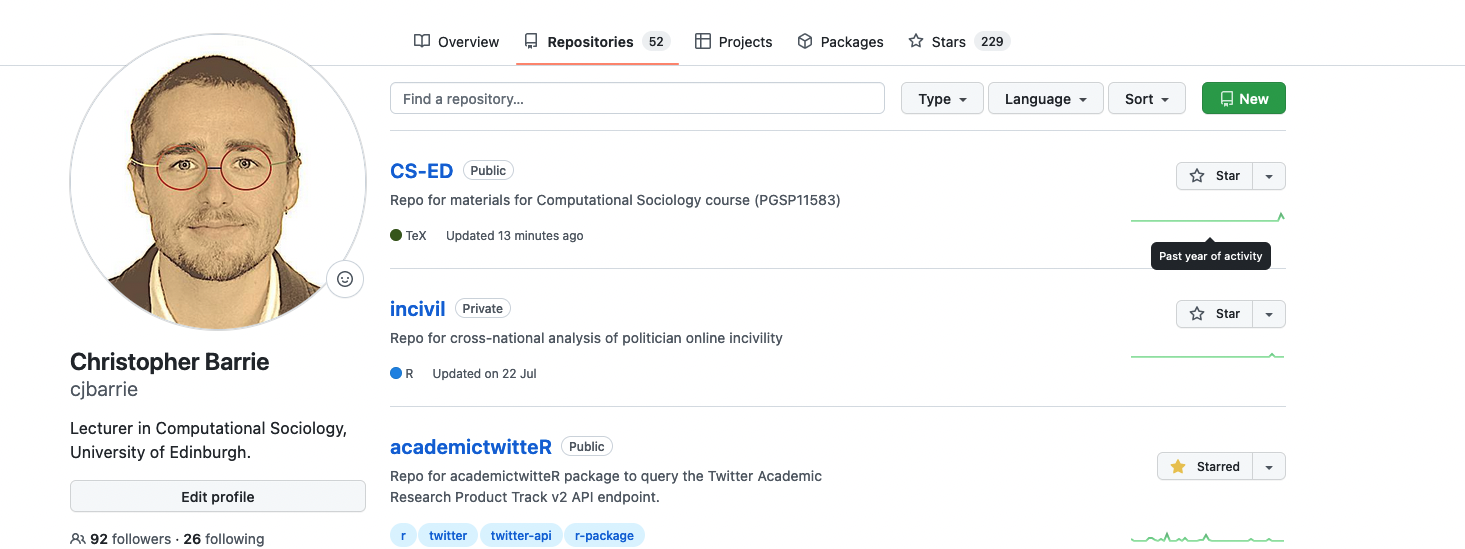
\includegraphics{./images/githubrepo.png}

Once you have created your Repo you can then get the files on your local
machine by calling the following:

\begin{Shaded}
\begin{Highlighting}[]
\ExtensionTok{$}\NormalTok{ git clone /path/to/repository}
\end{Highlighting}
\end{Shaded}

Where the path will just be the URL for your Repository.

\textbf{Additional tips} If you're unfamiliar with basic Git commands,
please refer to
\href{http://rogerdudler.GitHub.io/git-guide/files/git_cheat_sheet.pdf}{this
Git cheat sheet}.

\hypertarget{commit-changes}{%
\subsection*{Commit changes}\label{commit-changes}}
\addcontentsline{toc}{subsection}{Commit changes}

These features show how Git works as a version control system.

If you edited files or added new ones, you need to update your
repository. In Git terms, this action is called committing changes.

My current pwd is \texttt{CS-ED}. I created a text file named
\texttt{test} containing text \texttt{chris.} You can check the file
exists by typing `find ``test```.

The following is a typical workflow to reflect this change to the
remote.

\begin{Shaded}
\begin{Highlighting}[]
\ExtensionTok{$}\NormalTok{ git status }\CommentTok{\# check what\textquotesingle{}s changed. }
\ExtensionTok{$}\NormalTok{ git add . }\CommentTok{\# update every change. In Git terms, you\textquotesingle{}re staging. }
\ExtensionTok{$}\NormalTok{ git add file\_name }\CommentTok{\# or stage a specific file.}
\ExtensionTok{$}\NormalTok{ git commit }\AttributeTok{{-}m} \StringTok{"your comment"} \CommentTok{\# your comment for the commit. }
\ExtensionTok{$}\NormalTok{ git push origin main }\CommentTok{\# commit the change. Origin is a default name given to a server by Git. \textasciigrave{}origin main\textasciigrave{} are optional. }
\end{Highlighting}
\end{Shaded}

Another image from \href{https://git-scm.com/about/staging-area}{Pro
Git} nicely illustrates this process.

\begin{figure}

{\centering \includegraphics{https://git-scm.com/images/about/index1@2x.png}

}

\caption{Git Workflow}

\end{figure}

If you made a mistake, don't panic. You can't revert the process.

\begin{Shaded}
\begin{Highlighting}[]
\FunctionTok{git}\NormalTok{ reset }\AttributeTok{{-}{-}soft}\NormalTok{ HEAD\textasciitilde{}1 }\CommentTok{\# if you still want to keep the change, but you go back to t{-}1 }
\FunctionTok{git}\NormalTok{ reset }\AttributeTok{{-}{-}hard}\NormalTok{ HEAD\textasciitilde{}1 }\CommentTok{\# if you\textquotesingle{}re sure the change is unnecessary }
\end{Highlighting}
\end{Shaded}

Writing an informative commit is essential. To learn how to do this
better, see the following video:

\hypertarget{push-and-pull-or-fetch}{%
\subsection*{Push and pull (or fetch)}\label{push-and-pull-or-fetch}}
\addcontentsline{toc}{subsection}{Push and pull (or fetch)}

These features show how Git works as a collaboration tool.

If you have not already done it, let's clone the PS239T directory on
your local machine.

\begin{Shaded}
\begin{Highlighting}[]
\ExtensionTok{$}\NormalTok{ git clone https://github.com/PS239T/spring\_2021 }\CommentTok{\# clone }
\end{Highlighting}
\end{Shaded}

\textbf{Additional tips 1}

If you try to remove \texttt{spring\_2021} using
\texttt{rm\ -r\ spring\_2021/}, you will get an error about the
write-protected regular file. Then, try \texttt{rm\ -rf\ spring\_2021/}.

Then, let's learn more about the repository.

\begin{Shaded}
\begin{Highlighting}[]
\ExtensionTok{$}\NormalTok{ git remote }\AttributeTok{{-}v} 
\end{Highlighting}
\end{Shaded}

You should see something like the following:

\begin{Shaded}
\begin{Highlighting}[]
\ExtensionTok{origin}\NormalTok{  git@github.com:PS239T/spring\_2021 }\ErrorTok{(}\ExtensionTok{fetch}\KeywordTok{)}
\ExtensionTok{origin}\NormalTok{  git@github.com:PS239T/spring\_2021 }\ErrorTok{(}\ExtensionTok{push}\KeywordTok{)}
\end{Highlighting}
\end{Shaded}

If you want to see more information, then type
\texttt{git\ remote\ show\ origin.}

Previously, we learned how to send your data to save in the local
machine to the remote (the GitHub server). You can do that by editing or
creating files, committing, and typing \textbf{git push}.

Instead, if you want to update your local data with the remote data, you
can type \textbf{git pull origin} (something like pwd in bash).
Alternatively, you can use fetch (retrieve data from a remote). Git
retrieves the data and merges it into your local data when you do that.

\begin{Shaded}
\begin{Highlighting}[]
\ExtensionTok{$}\NormalTok{ git fetch origin}
\end{Highlighting}
\end{Shaded}

\textbf{Additional tips 2}

Developers usually use PR to refer pull requests. When you are making
PRs, it's recommended to scope down (small PRs) because they are easier
on reviewers and to test. To learn about how to accomplish this, see
\href{https://www.netlify.com/blog/2020/03/31/how-to-scope-down-prs/}{this
blog post} by Sarah Drasner.

\hypertarget{branching}{%
\subsection*{Branching}\label{branching}}
\addcontentsline{toc}{subsection}{Branching}

It's an advanced feature of Git's version control system that allows
developers to ``diverge from the main line of development and continue
to do work without messing with that main line,'' according to
\href{https://git-scm.com/book/en/v1/Git-Branching}{Scott Chacon and Ben
Straub}.

If you start working on a new feature, create a new branch.

\begin{Shaded}
\begin{Highlighting}[]
\ExtensionTok{$}\NormalTok{ git branch new\_features}
\ExtensionTok{$}\NormalTok{ git checkout new\_features}
\end{Highlighting}
\end{Shaded}

You can see the newly created branch by typing \textbf{git branch}.

In short, branching makes Git
\href{https://git-scm.com/book/en/v2/Getting-Started-Git-Basics}{works
like} a mini file system.

\hypertarget{other-useful-commands}{%
\subsection*{Other useful commands}\label{other-useful-commands}}
\addcontentsline{toc}{subsection}{Other useful commands}

\begin{enumerate}
\def\labelenumi{\arabic{enumi}.}
\tightlist
\item
  For tracking history
\end{enumerate}

\begin{Shaded}
\begin{Highlighting}[]
\ExtensionTok{$}\NormalTok{ git diff }\CommentTok{\# to see what changed (e.g., inside a file)}
\ExtensionTok{$}\NormalTok{ git log }\CommentTok{\# to track who committed what}
\ExtensionTok{$}\NormalTok{ git log }\AttributeTok{{-}S} \OperatorTok{\textless{}}\NormalTok{pattern}\OperatorTok{\textgreater{}}\NormalTok{ \# you can find a log that contains the pattern }
\ExtensionTok{$}\NormalTok{ git checkout }\CommentTok{\# to recover old files }
\ExtensionTok{$}\NormalTok{ git revert }\CommentTok{\# revert to the previous commit }
\end{Highlighting}
\end{Shaded}

\begin{enumerate}
\def\labelenumi{\arabic{enumi}.}
\setcounter{enumi}{1}
\tightlist
\item
  For removing and renaming files
\end{enumerate}

\begin{Shaded}
\begin{Highlighting}[]
\ExtensionTok{$}\NormalTok{ git rm file\_name }\CommentTok{\# remove }
\ExtensionTok{$}\NormalTok{ git mv old\_file\_name new\_file\_name }\CommentTok{\# rename a file }
\end{Highlighting}
\end{Shaded}

How about removing a directory only from GitHub but not local?

\begin{Shaded}
\begin{Highlighting}[]
\FunctionTok{git}\NormalTok{ rm }\AttributeTok{{-}r} \AttributeTok{{-}{-}cached} \OperatorTok{\textless{}}\NormalTok{directory}\OperatorTok{\textgreater{}}
\FunctionTok{git}\NormalTok{ commit }\AttributeTok{{-}m} \StringTok{"\textless{}message\textgreater{}"}
\FunctionTok{git}\NormalTok{ push}
\end{Highlighting}
\end{Shaded}

\hypertarget{collaborations}{%
\subsection*{Collaborations}\label{collaborations}}
\addcontentsline{toc}{subsection}{Collaborations}

Two options.

\begin{itemize}
\tightlist
\item
  Sharing a repository (suitable for a private project).
\item
  Fork and pull (suitable for an open-source project). \hspace{0pt} *
  The one who maintains the repository becomes the maintainer.
  \hspace{0pt} * The others can
  \href{https://help.GitHub.com/articles/about-forks/}{fork}, make
  changes, and even
  \href{https://help.GitHub.com/articles/about-pull-requests/}{pull}
  them back.
\end{itemize}

\hypertarget{deployment-github-pages}{%
\subsection*{Deployment: GitHub Pages}\label{deployment-github-pages}}
\addcontentsline{toc}{subsection}{Deployment: GitHub Pages}

Useful to deploy websites. I used the GitHub page to deploy this book.

\hypertarget{tracking-progress-github-issues}{%
\subsection*{Tracking progress: GitHub
Issues}\label{tracking-progress-github-issues}}
\addcontentsline{toc}{subsection}{Tracking progress: GitHub Issues}

Useful to collect and respond to questions and suggestions (e.g., bug
reports and feature suggestions) on the projects on which you're
working.

\hypertarget{project-management-github-dashboards}{%
\subsection*{Project management: GitHub
Dashboards}\label{project-management-github-dashboards}}
\addcontentsline{toc}{subsection}{Project management: GitHub Dashboards}

I use GitHub dashboards for almost every project that I have done.

\hypertarget{the-big-picture-2}{%
\subsection*{The Big Picture}\label{the-big-picture-2}}
\addcontentsline{toc}{subsection}{The Big Picture}

When you are reading this section, please note that you've already
grasped some key concepts behind R programming language (functions and
objects).

UNIX Commands (\texttt{cat}) = R Functions (\texttt{print}) Files = R
Objects

\hypertarget{motivation}{%
\subsection*{Motivation}\label{motivation}}
\addcontentsline{toc}{subsection}{Motivation}

Why do you need to make your research computationally reproducible?: for
your own sanity and for public benefit. That is, it makes your life a
whole lot easier to have a history of what you've done and why. And it
makes research more transparent and reproducible: others can see what
you've done, how you've done it---and they can go off and build on this.

\hypertarget{how-to-organize-files-in-a-project}{%
\subsubsection*{How to organize files in a
project}\label{how-to-organize-files-in-a-project}}
\addcontentsline{toc}{subsubsection}{How to organize files in a project}

You won't be able to reproduce your project unless it is efficiently
organized.

Step 1. \href{https://environments.rstudio.com/}{\textbf{Environment}}
is part of your project. If someone can't reproduce your environment,
they won't be able to run your code.

\begin{itemize}
\tightlist
\item
  Launch R Studio. Tools \textgreater{} Global Options. You
  \textbf{should not} check Restore .RData into workspace at startup.
  Also, set the saving workspace option to \textbf{NEVER.}
\end{itemize}

Step 2. For each project, create a project directory named after the
project.

name\_of\_the\_project

\begin{itemize}
\tightlist
\item
  01\_script\_that\_does\_first\_thing.R
\item
  02\_script\_that\_does\_second\_thing.R
\item
  data:

  \begin{itemize}
  \tightlist
  \item
    raw
  \item
    processed (all processed, cleaned, and tided)
  \end{itemize}
\item
  figures
\item
  functions
\item
  reports (PDF, HTML, TEX, etc.,)
\item
  results (model outcomes, etc.,)
\item
  .gitignore (for Git)
\item
  name\_of\_project.Rproj (for R)
\item
  README.md (for Git)
\end{itemize}

\begin{Shaded}
\begin{Highlighting}[]
\CommentTok{\# Don\textquotesingle{}t name it a project. Instead, use a more informative name. For instance, \textasciigrave{}us\_election\textasciigrave{}, not \textasciigrave{}my\_project.\textasciigrave{}}

\FunctionTok{dir.create}\NormalTok{(}\StringTok{"../us\_election"}\NormalTok{)}
\end{Highlighting}
\end{Shaded}

Step 3. Launch R Studio. Choose File \textgreater{} New project
\textgreater{} Browse existing directories \textgreater{} Create
project. This means each project has its own workspace.

Step 4. Organize files by putting them in separate subdirectories and
sensibly naming them.

\begin{itemize}
\item
  Treat raw data as read-only (raw data should be RAW!) and put it in
  the \texttt{data} subdirectory.

  \begin{itemize}
  \tightlist
  \item
    Again, note that version control does not need to replace backup.
    You still need to back up your raw data.
  \end{itemize}
\end{itemize}

\begin{Shaded}
\begin{Highlighting}[]
\FunctionTok{dir.create}\NormalTok{(here}\SpecialCharTok{::}\FunctionTok{here}\NormalTok{(}\StringTok{"us\_election"}\NormalTok{, }\StringTok{"data"}\NormalTok{))}
\end{Highlighting}
\end{Shaded}

And separate into \texttt{raw} and \texttt{processed}

\begin{Shaded}
\begin{Highlighting}[]
\FunctionTok{dir.create}\NormalTok{(here}\SpecialCharTok{::}\FunctionTok{here}\NormalTok{(}\StringTok{"us\_election/data/"}\NormalTok{, }\StringTok{"raw"}\NormalTok{))}
\FunctionTok{dir.create}\NormalTok{(here}\SpecialCharTok{::}\FunctionTok{here}\NormalTok{(}\StringTok{"us\_election/data/"}\NormalTok{, }\StringTok{"processed"}\NormalTok{))}
\end{Highlighting}
\end{Shaded}

\begin{itemize}
\tightlist
\item
  Separate figures into the \texttt{figures} subdirectory.
\end{itemize}

\begin{Shaded}
\begin{Highlighting}[]
\FunctionTok{dir.create}\NormalTok{(here}\SpecialCharTok{::}\FunctionTok{here}\NormalTok{(}\StringTok{"us\_election"}\NormalTok{, }\StringTok{"figures"}\NormalTok{))}
\end{Highlighting}
\end{Shaded}

\begin{itemize}
\tightlist
\item
  Put any reports in the \texttt{reports} subdirectory.
\end{itemize}

\begin{Shaded}
\begin{Highlighting}[]
\FunctionTok{dir.create}\NormalTok{(here}\SpecialCharTok{::}\FunctionTok{here}\NormalTok{(}\StringTok{"us\_election"}\NormalTok{, }\StringTok{"reports"}\NormalTok{))}
\end{Highlighting}
\end{Shaded}

\begin{itemize}
\tightlist
\item
  Put generated results in the `results`` subdirectory and treat them as
  disposable.
\end{itemize}

\begin{Shaded}
\begin{Highlighting}[]
\FunctionTok{dir.create}\NormalTok{(here}\SpecialCharTok{::}\FunctionTok{here}\NormalTok{(}\StringTok{"us\_election"}\NormalTok{, }\StringTok{"results"}\NormalTok{))}
\end{Highlighting}
\end{Shaded}

\begin{itemize}
\tightlist
\item
  Put your custom functions in the \texttt{functions} subdirectory.
\end{itemize}

\begin{Shaded}
\begin{Highlighting}[]
\FunctionTok{dir.create}\NormalTok{(here}\SpecialCharTok{::}\FunctionTok{here}\NormalTok{(}\StringTok{"us\_election"}\NormalTok{, }\StringTok{"functions"}\NormalTok{))}
\end{Highlighting}
\end{Shaded}

Are you tired of creating these directories one by one? Why not
automate? See the following example. You can save this function as a
rscript (e.g., \texttt{setup.r}) and run it in the terminal using
\texttt{Rscript\ \textless{}script\ name\textgreater{}.}

\begin{Shaded}
\begin{Highlighting}[]
\ControlFlowTok{if}\NormalTok{ (}\SpecialCharTok{!}\FunctionTok{require}\NormalTok{(pacman)) }\FunctionTok{install.packages}\NormalTok{(}\StringTok{"pacman"}\NormalTok{)}

\CommentTok{\# Load here}
\NormalTok{pacman}\SpecialCharTok{::}\FunctionTok{p\_load}\NormalTok{(}
\NormalTok{  purrr, }\CommentTok{\# functional programming}
\NormalTok{  here }\CommentTok{\# computational reproducibility}
\NormalTok{)}

\CommentTok{\# Custom function}
\NormalTok{create\_dirs }\OtherTok{\textless{}{-}} \ControlFlowTok{function}\NormalTok{(name) \{}
  \FunctionTok{dir.create}\NormalTok{(}\FunctionTok{here}\NormalTok{(name))}
\NormalTok{\}}

\CommentTok{\# Apply function }
\NormalTok{purrr}\SpecialCharTok{::}\FunctionTok{map}\NormalTok{(}\FunctionTok{c}\NormalTok{(}\StringTok{"data"}\NormalTok{, }\StringTok{"figures"}\NormalTok{, }\StringTok{"reports"}\NormalTok{, }\StringTok{"results"}\NormalTok{, }\StringTok{"functions"}\NormalTok{), create\_dirs)}
\end{Highlighting}
\end{Shaded}

Of course, you don't have to use these exact names. But here's an
example of how I tend to structure my directories---and you'll see it
follows this basic structure.

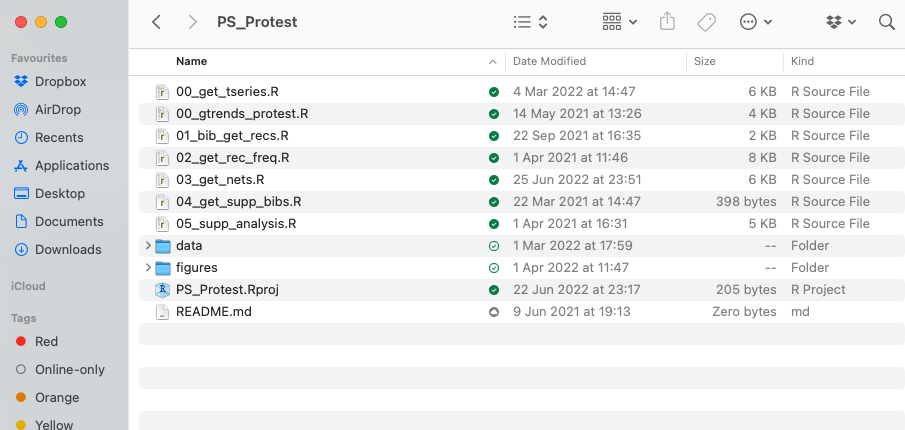
\includegraphics{./images/direx.png}

\hypertarget{how-to-organize-code-in-an-r-markdown-file}{%
\subsection*{How to organize code in an R markdown
file}\label{how-to-organize-code-in-an-r-markdown-file}}
\addcontentsline{toc}{subsection}{How to organize code in an R markdown
file}

\begin{itemize}
\item
  In addition to environment, \textbf{workflow} is an essential
  component of project efficiency and reproducibility.
\item
  What is R markdown? An R package, developed by
  \href{https://yihui.org/en/}{Yihui Xie}, provides an authoring
  framework for data science. Xie is also a developer of many widely
  popular R packages such as \texttt{knitr,}
  \href{https://GitHub.com/yihui/xaringan}{\texttt{xaringan}} (cool kids
  use xaringan not
  \href{https://en.wikipedia.org/wiki/Beamer_(LaTeX)}{Beamer} these
  days), \texttt{blogdown} (used to create
  \href{https://jaeyk.GitHub.io/}{my personal website}), and
  \texttt{bookdown} (used to create this book) among many others.

  \begin{itemize}
  \tightlist
  \item
    Many applications:
    \href{https://rstudio.GitHub.io/distill/basics.html}{reports},
    \href{https://bookdown.org/yihui/rmarkdown/xaringan.html}{presentations},
    \href{https://rmarkdown.rstudio.com/flexdashboard/}{dashboards},
    \href{https://bookdown.org/yihui/rmarkdown/websites.html}{websites}\\
  \item
    Check out \href{https://ysc-rmarkdown.netlify.app/}{Communicating
    with R markdown workshop} by \href{https://alison.rbind.io/}{Alison
    Hill} (RStudio)

    \begin{itemize}
    \tightlist
    \item
      Alison Hill is a co-author of
      \href{https://bookdown.org/yihui/blogdown/}{\texttt{blogdown:\ Creating\ Websites\ with\ R\ Markdown.}}
    \end{itemize}
  \item
    Key strengths: dynamic reporting + reproducible science + easy
    deployment
  \end{itemize}
\end{itemize}

\begin{figure}

{\centering \includegraphics{https://GitHub.com/rstudio/concept-maps/raw/master/en/rmarkdown.svg}

}

\caption{Concept map for R Markdown. By Gabriela Sandoval, Florencia
D'Andrea, Yanina Bellini Saibene, Monica Alonso.}

\end{figure}

\begin{itemize}
\tightlist
\item
  R Markdown basic syntax
\end{itemize}

\begin{Shaded}
\begin{Highlighting}[]
\CommentTok{\# Header 1}
\DocumentationTok{\#\# Header 2}
\DocumentationTok{\#\#\# Header 3}
\end{Highlighting}
\end{Shaded}

\begin{itemize}
\tightlist
\item
  Use these section headers to indicate workflow.
\end{itemize}

\begin{Shaded}
\begin{Highlighting}[]
\CommentTok{\# Import packages and data}
\CommentTok{\# Tidy data}
\CommentTok{\# Wrangle data}
\CommentTok{\# Model data}
\CommentTok{\# Visualize data}
\end{Highlighting}
\end{Shaded}

Press \texttt{ctrl\ +\ shift\ +\ o}. You can see a document outline
based on these headers. This is a nice feature for finding the code you
need to focus on.

If your project's scale is large, divide these sections into files and
numbers and save them in the \texttt{code} subdirectory.

\begin{itemize}
\tightlist
\item
  01\_wrangling.Rmd
\item
  02\_modeling.Rmd \ldots{}
\end{itemize}

\hypertarget{making-a-project-computationally-reproducible}{%
\subsubsection*{Making a project computationally
reproducible}\label{making-a-project-computationally-reproducible}}
\addcontentsline{toc}{subsubsection}{Making a project computationally
reproducible}

\begin{itemize}
\item
  \texttt{setwd()}: set a working directory.
\item
  Note that using \texttt{setwd()} is not a reproducible way to set up
  your project. For instance, none will be able to run the following
  code except me.
\end{itemize}

\begin{Shaded}
\begin{Highlighting}[]
\CommentTok{\# Set a working directory }
\FunctionTok{setwd}\NormalTok{(}\StringTok{"/home/jae/starwars"}\NormalTok{)}

\CommentTok{\# Do something }
\FunctionTok{ggplot}\NormalTok{(mtcars, }\FunctionTok{aes}\NormalTok{(}\AttributeTok{x =}\NormalTok{ mpg, }\AttributeTok{y =}\NormalTok{ wt)) }\SpecialCharTok{+}
   \FunctionTok{geom\_point}\NormalTok{()}

\CommentTok{\# Export the object. }
\CommentTok{\# dot means the working directory set by setwd()}
\FunctionTok{ggsave}\NormalTok{(}\StringTok{"./outputs/example.png"}\NormalTok{) }\CommentTok{\# This is called relative path }
\end{Highlighting}
\end{Shaded}

\begin{itemize}
\item
  Instead, learn how to use \texttt{here()}'.

  \begin{itemize}
  \item
    Key idea: separate workflow (e.g., workspace information) from
    products (code and data). For more information, please read Jenny
    Bryan's excellent piece on
    \href{https://www.tidyverse.org/blog/2017/12/workflow-vs-script/}{project-oriented
    workflow}.
  \item
    Example
  \end{itemize}
\end{itemize}

\begin{Shaded}
\begin{Highlighting}[]
\CommentTok{\# New: Reproducible }

\FunctionTok{ggplot}\NormalTok{(mtcars, }\FunctionTok{aes}\NormalTok{(}\AttributeTok{x =}\NormalTok{ mpg, }\AttributeTok{y =}\NormalTok{ wt)) }\SpecialCharTok{+}
   \FunctionTok{geom\_point}\NormalTok{()}

\FunctionTok{ggsave}\NormalTok{(}\FunctionTok{here}\NormalTok{(}\StringTok{"project"}\NormalTok{, }\StringTok{"outputs"}\NormalTok{, }\StringTok{"example.png"}\NormalTok{))}
\end{Highlighting}
\end{Shaded}

\begin{itemize}
\tightlist
\item
  How \texttt{here} works
\end{itemize}

\texttt{here()} function shows what's the top-level project directory.

\begin{Shaded}
\begin{Highlighting}[]
\NormalTok{here}\SpecialCharTok{::}\FunctionTok{here}\NormalTok{()}
\end{Highlighting}
\end{Shaded}

\begin{itemize}
\tightlist
\item
  Build a path including subdirectories
\end{itemize}

\begin{Shaded}
\begin{Highlighting}[]
\NormalTok{here}\SpecialCharTok{::}\FunctionTok{here}\NormalTok{(}\StringTok{"project"}\NormalTok{, }\StringTok{"outputs"}\NormalTok{)}
           \CommentTok{\#depth 1   \#depth 2}
\end{Highlighting}
\end{Shaded}

\begin{itemize}
\item
  How \texttt{here} defines the top-level project directory. For
  example, the following list came from
  \href{https://GitHub.com/jennybc/here_here}{the here package
  vignette}).

  \begin{itemize}
  \item
    Is a file named .here present?
  \item
    Is this an RStudio Project? (\textbf{Note that we already set up an
    RStudio Project!} So, if you use RStudio's project feature, then you
    are ready to use \texttt{here}.)
  \item
    Is this an R package? Does it have a DESCRIPTION file?
  \item
    Is this a remake project? Does it have a file named
    \texttt{remake.yml}?
  \item
    Is this a projectile project? Does it have a file named
    \texttt{.projectile}?
  \item
    Is this a checkout from a version control system? Does it have a
    directory named \texttt{.git} or \texttt{.svn}? Currently, only Git
    and Subversion are supported.
  \item
    If there's no match then use \texttt{set\_here()} to create an empty
    \texttt{.here} file.
  \end{itemize}
\end{itemize}

\hypertarget{references-1}{%
\subsection*{References}\label{references-1}}
\addcontentsline{toc}{subsection}{References}

\begin{itemize}
\item
  Code and data management

  \begin{itemize}
  \tightlist
  \item
    \href{https://web.stanford.edu/~gentzkow/research/CodeAndData.pdf}{``Code
    and Data for the Social Sciences: A Practitioner's Guide''} by
    Matthew Gentkow and Jesse M. Shapiro
  \end{itemize}
\item
  Project-oriented research

  \begin{itemize}
  \item
    Computational reproducibility

    \begin{itemize}
    \item
      \href{https://GitHub.com/swcarpentry/good-enough-practices-in-scientific-computing/blob/gh-pages/good-enough-practices-for-scientific-computing.pdf}{``Good
      Enough Practices in Scientific Computing''} by PLOS
    \item
      \href{https://swcarpentry.GitHub.io/r-novice-gapminder/02-project-intro/}{Project
      Management with RStudio} by Software Carpentry
    \item
      \href{https://kbroman.org/steps2rr/}{Initial steps toward
      reproducible research} by Karl Broman
    \end{itemize}
  \item
    Version control

    \begin{itemize}
    \item
      \href{https://swcarpentry.GitHub.io/git-novice/}{Version Control
      with Git} by Software Carpentry
    \item
      \href{http://plain-text.co/}{The Plain Person's Guide to Plain
      Text Social Science} by Kieran Healy
    \end{itemize}
  \end{itemize}
\end{itemize}

\bookmarksetup{startatroot}

\hypertarget{introduction-to-r}{%
\chapter*{Introduction to R}\label{introduction-to-r}}
\addcontentsline{toc}{chapter}{Introduction to R}

This section is designed to ensure you are familiar with the R
environment.

\hypertarget{getting-started-with-r-at-home}{%
\section*{Getting started with R at
home}\label{getting-started-with-r-at-home}}
\addcontentsline{toc}{section}{Getting started with R at home}

Given that we're all working from home these days, you'll need to
download R and RStudio onto your own devices. R is the name of the
programming language that we'll be using for coding exercises; RStudio
is the IDE (``Integrated Development Environment''), i.e., the piece of
software that almost everyone uses when working in R.

You can download both of these on Windows and Mac easily and for free.
This is one of the first reasons to use an ``open-source'' programming
language: it's free and everyone can contribute!

IT Services at the University of Edinburgh have provided a
\href{https://uoe.sharepoint.com/sites/hss/sps/itservices/SPSShareSpaceManagement/Moblabdoc/SitePages/Computational-Text-Analysis.aspx?cid=59b29656-3df8-4c19-9423-24765076e742}{walkthrough}
of what is needed for you to get started. I also break this down below:

\begin{enumerate}
\def\labelenumi{\arabic{enumi}.}
\item
  Install R for Mac from here: https://cran.r-project.org/bin/macosx/.
  Install R for Windows from here:
  https://cran.r-project.org/bin/windows/base/.
\item
  Download RStudio for Windows or Mac from here:
  https://rstudio.com/products/rstudio/download/, choosing the Free
  version: this is what most people use and is more than enough for all
  of our needs.
\end{enumerate}

\textbf{All programs are free. Make sure to load everything listed above
for your operating system or R will not work properly!}

\hypertarget{some-basic-information}{%
\section*{Some basic information}\label{some-basic-information}}
\addcontentsline{toc}{section}{Some basic information}

\begin{itemize}
\item
  A script is a text file in which you write your commands (code) and
  comments.
\item
  If you put the \# character in front of a line of text this line will
  not be executed; this is useful to add comments to your script!
\item
  R is case sensitive, so be careful when typing.
\item
  To send code from the script to the console, highlight the relevant
  line of code in your script and click on Run, or select the line and
  hit ctrl+enter on PCR or cmd+enter on Mac
\item
  Access help files for R functions by preceding the name of the
  function with ? (e.g., ?table)
\item
  By pressing the up key, you can go back to the commands you have used
  before
\item
  Press the tab key to auto-complete variable names and commands
\end{itemize}

\hypertarget{getting-started-in-rstudio}{%
\section*{Getting Started in RStudio}\label{getting-started-in-rstudio}}
\addcontentsline{toc}{section}{Getting Started in RStudio}

Begin by opening RStudio (located on the desktop). Your first task is to
create a new script (this is where we will write our commands). To do
so, click:

\begin{Shaded}
\begin{Highlighting}[]
\NormalTok{File }\SpecialCharTok{{-}}\OtherTok{{-}\textgreater{}}\NormalTok{ NewFile }\SpecialCharTok{{-}}\OtherTok{{-}\textgreater{}}\NormalTok{ RScript}
\end{Highlighting}
\end{Shaded}

Your screen should now have four panes:

\begin{itemize}
\item
  the Script (top left)
\item
  the Console (bottom left)
\item
  the Environment/History (top right)
\item
  Files/Plots/Packages/Help/Viewer (bottom right)
\end{itemize}

\hypertarget{a-simple-example}{%
\section*{A simple example}\label{a-simple-example}}
\addcontentsline{toc}{section}{A simple example}

The Script (top left) is where we write our commands for R. You can try
this out for a first time by writing a small snipped of code as follows:

\begin{Shaded}
\begin{Highlighting}[]
\NormalTok{x }\OtherTok{\textless{}{-}} \StringTok{"I can\textquotesingle{}t wait to learn Computational Text Analysis"} \CommentTok{\#Note the quotation marks!}
\end{Highlighting}
\end{Shaded}

To tell R to run the command, highlight the relevant row in your script
and click the Run button (top right of the Script) - or hold down
ctrl+enter on Windows or cmd+enter on Mac - to send the command to the
Console (bottom left), where the actual evaluation and calculations are
taking place. These shortcut keys will become very familiar to you very
quickly!

Running the command above creates an object named `x', that contains the
words of your message.

You can now see `x' in the Environment (top right). To view what is
contained in x, type in the Console (bottom left):

\begin{Shaded}
\begin{Highlighting}[]
\FunctionTok{print}\NormalTok{(x)}
\end{Highlighting}
\end{Shaded}

\begin{verbatim}
[1] "I can't wait to learn Computational Text Analysis"
\end{verbatim}

\begin{Shaded}
\begin{Highlighting}[]
\CommentTok{\# or alternatively you can just type:}

\NormalTok{x}
\end{Highlighting}
\end{Shaded}

\begin{verbatim}
[1] "I can't wait to learn Computational Text Analysis"
\end{verbatim}

\hypertarget{loading-packages}{%
\section*{Loading packages}\label{loading-packages}}
\addcontentsline{toc}{section}{Loading packages}

The `base' version of R is very powerful but it will not be able to do
everything on its own, at least not with ease. For more technical or
specialized forms of analysis, we will need to load new packages.

This is when we will need to install a so-called `package'---a program
that includes new tools (i.e., functions) to carry out specific tasks.
You can think of them as `extensions' enhancing R's capacities.

To take one example, we might want to do something a little more
exciting than print how excited we are about this course. Let's make a
map instead.

This might sound technical. But the beauty of the packaged extensions of
R is that they contain functions to perform specialized types of
analysis with ease.

We'll first need to install one of these packages, which you can do as
below:

\begin{Shaded}
\begin{Highlighting}[]
\FunctionTok{install.packages}\NormalTok{(}\StringTok{"tidyverse"}\NormalTok{)}
\end{Highlighting}
\end{Shaded}

After the package is installed, we then need to load it into our
environment by typing library(). Note that, here, you don't need to wrap
the name of the package in quotation marks. So this will do the trick:

\begin{Shaded}
\begin{Highlighting}[]
\FunctionTok{library}\NormalTok{(tidyverse)}
\end{Highlighting}
\end{Shaded}

\begin{verbatim}
-- Attaching packages --------------------------------------- tidyverse 1.3.1 --
\end{verbatim}

\begin{verbatim}
v ggplot2 3.3.6     v purrr   0.3.4
v tibble  3.1.7     v dplyr   1.0.9
v tidyr   1.2.0     v stringr 1.4.0
v readr   2.1.2     v forcats 0.5.1
\end{verbatim}

\begin{verbatim}
-- Conflicts ------------------------------------------ tidyverse_conflicts() --
x dplyr::filter() masks stats::filter()
x dplyr::lag()    masks stats::lag()
\end{verbatim}

What now? Well, let's see just how easy it is to visualize some data
using ggplot which is a package that comes bundled into the larger
tidyverse package.

\begin{Shaded}
\begin{Highlighting}[]
\FunctionTok{ggplot}\NormalTok{(}\AttributeTok{data =}\NormalTok{ mpg) }\SpecialCharTok{+} 
  \FunctionTok{geom\_point}\NormalTok{(}\AttributeTok{mapping =} \FunctionTok{aes}\NormalTok{(}\AttributeTok{x =}\NormalTok{ displ, }\AttributeTok{y =}\NormalTok{ hwy))}
\end{Highlighting}
\end{Shaded}

\begin{figure}[H]

{\centering 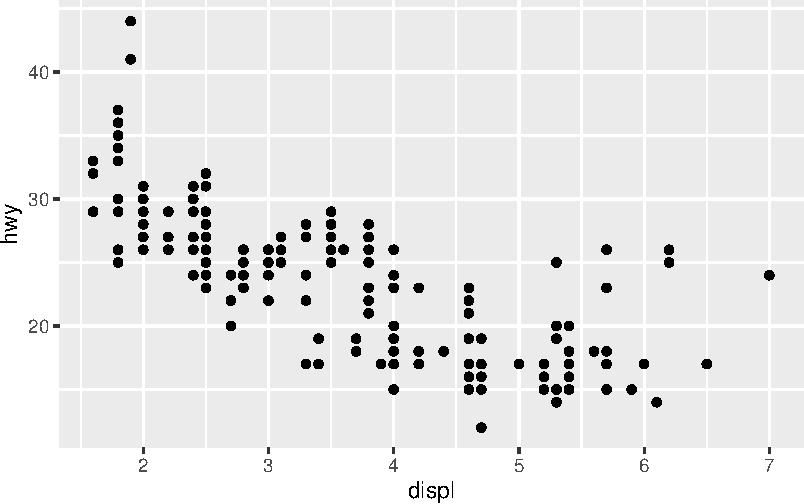
\includegraphics{./intror_files/figure-pdf/unnamed-chunk-12-1.pdf}

}

\end{figure}

If we wanted to save where we'd got to with making our plots, we would
want to save our scripts, and maybe the data we used as well, so that we
could return to it at a later stage.

\hypertarget{saving-your-objects-plots-and-scripts}{%
\section*{Saving your objects, plots and
scripts}\label{saving-your-objects-plots-and-scripts}}
\addcontentsline{toc}{section}{Saving your objects, plots and scripts}

\begin{itemize}
\item
  Saving scripts: To save your script in RStudio (i.e.~the top left
  panel), all you need to do is click File --\textgreater{} Save As (and
  choose a name for your script). Your script will be something like:
  myfilename.R.
\item
  Saving plots: If you have made any plots you would like to save, click
  Export (in the plotting pane) and choose a relevant file extension
  (e.g.~.png, .pdf, etc.) and size.
\item
  To save \textbf{individual} objects (for example x from above) from
  your environment, run the following command (choosing a suitable
  filename):
\end{itemize}

\begin{Shaded}
\begin{Highlighting}[]
\FunctionTok{save}\NormalTok{(x,}\AttributeTok{file=}\StringTok{"myobject.RData"}\NormalTok{)}
\FunctionTok{load}\NormalTok{(}\AttributeTok{file=}\StringTok{"myobject.RData"}\NormalTok{)}
\end{Highlighting}
\end{Shaded}

\begin{itemize}
\tightlist
\item
  To save \textbf{all} of your objects (i.e.~everything in the top right
  panel) at once, run the following command (choosing a suitable
  filename):
\end{itemize}

\begin{Shaded}
\begin{Highlighting}[]
\FunctionTok{save.image}\NormalTok{(}\AttributeTok{file=}\StringTok{"myfilname.RData"}\NormalTok{)}
\end{Highlighting}
\end{Shaded}

\begin{itemize}
\tightlist
\item
  Your objects can be re-loaded into R during your next session by
  running:
\end{itemize}

\begin{Shaded}
\begin{Highlighting}[]
\FunctionTok{load}\NormalTok{(}\AttributeTok{file=}\StringTok{"myfilename.RData"}\NormalTok{)}
\end{Highlighting}
\end{Shaded}

There are many other file formats you might use to save any output. We
will encounter these as the course progresses.

\hypertarget{knowing-where-r-saves-your-documents}{%
\section*{Knowing where R saves your
documents}\label{knowing-where-r-saves-your-documents}}
\addcontentsline{toc}{section}{Knowing where R saves your documents}

If you are at home, when you open a new script make sure to check and
set your working directory (i.e.~the folder where the files you create
will be saved). To check your working directory use the getwd() command
(type it into the Console or write it in your script in the Source
Editor):

\begin{Shaded}
\begin{Highlighting}[]
\FunctionTok{getwd}\NormalTok{()}
\end{Highlighting}
\end{Shaded}

To set your working directory, run the following command, substituting
the file directory of your choice. Remember that anything following the
`\#' symbol is simply a clarifying comment and R will not process it.

\begin{Shaded}
\begin{Highlighting}[]
\DocumentationTok{\#\# Example for Mac }
\FunctionTok{setwd}\NormalTok{(}\StringTok{"/Users/Documents/mydir/"}\NormalTok{) }
\DocumentationTok{\#\# Example for PC }
\FunctionTok{setwd}\NormalTok{(}\StringTok{"c:/docs/mydir"}\NormalTok{) }
\end{Highlighting}
\end{Shaded}

\hypertarget{practicing-in-r}{%
\section*{Practicing in R}\label{practicing-in-r}}
\addcontentsline{toc}{section}{Practicing in R}

The best way to learn R is to use it. These workshops on text analysis
will not be the place to become fully proficient in R. They will,
however, be a chance to conduct some hands-on analysis with applied
examples in a fast-expanding field. And the best way to learn is through
doing. So give it a shot!

For some further practice in the R programming language, look no further
than Wickham and Grolemund (2017) and, for tidy text analysis, Silge and
Robinson (2017).

\begin{itemize}
\item
  The free online book by Hadley Wickham ``R for Data Science'' is
  available \href{https://r4ds.had.co.nz/}{here}
\item
  The free online book by Julia Silge and David Robinson ``Text Mining
  with R'' is available \href{https://www.tidytextmining.com/}{here}
\item
  For more practice with R, you may want to consult a set of interactive
  tutorials, available through the package ``learnr.'' Once you've
  installed this package, you can go through the tutorials yourselves by
  calling:
\end{itemize}

\begin{Shaded}
\begin{Highlighting}[]
\FunctionTok{library}\NormalTok{(learnr)}

\FunctionTok{available\_tutorials}\NormalTok{() }\CommentTok{\# this will tell you the names of the tutorials available}

\FunctionTok{run\_tutorial}\NormalTok{(}\AttributeTok{name =} \StringTok{"ex{-}data{-}basics"}\NormalTok{, }\AttributeTok{package =} \StringTok{"learnr"}\NormalTok{) }\CommentTok{\#this will launch the interactive tutorial in a new Internet browser window}
\end{Highlighting}
\end{Shaded}

\hypertarget{one-final-note}{%
\section*{One final note}\label{one-final-note}}
\addcontentsline{toc}{section}{One final note}

Once you've dipped into the ``R for Data Science'' book you'll hear a
lot about the so-called tidyverse in R. This is essentially a set of
packages that use an alternative, and more intuitive, way of interacting
with data.

The main difference you'll notice here is that, instead of having
separate lines for each function we want to run, or wrapping functions
inside functions, sets of functions are ``piped'' into each other using
``pipe'' functions, which look have the appearance:
\texttt{\%\textgreater{}\%}.

I will be using ``tidy'' syntax in the weekly exercises for these
computational text analysis workshops. If anything is unclear, I can
provide the equivalents in ``base'' R too. But a lot of the useful text
analysis packages are now composed with `tidy' syntax.

\bookmarksetup{startatroot}

\hypertarget{code-style-guide}{%
\chapter*{Code style guide}\label{code-style-guide}}
\addcontentsline{toc}{chapter}{Code style guide}

\begin{tcolorbox}[enhanced jigsaw, rightrule=.15mm, arc=.35mm, bottomrule=.15mm, colback=white, toprule=.15mm, breakable, left=2mm, colframe=quarto-callout-note-color-frame, leftrule=.75mm, opacityback=0]
\begin{minipage}[t]{5.5mm}
\textcolor{quarto-callout-note-color}{\faInfo}
\end{minipage}%
\begin{minipage}[t]{\textwidth - 5.5mm}
The following introductory section is taken, in slightly adapted form,
from Jae Yeon Kim's ``Computational Thinking for Social Scientists.'' It
is reproduced here for ease of access. To consult the full book, go to
\url{https://jaeyk.github.io/comp_thinking_social_science/}.\end{minipage}%
\end{tcolorbox}

\hypertarget{the-big-piture}{%
\section*{The Big Piture}\label{the-big-piture}}
\addcontentsline{toc}{section}{The Big Piture}

\begin{itemize}
\tightlist
\item
  What is code style?
\end{itemize}

\begin{quote}
Every major open-source project has its style guide: a set of
conventions (sometimes arbitrary) about writing code for that project.
It is much easier to understand a large codebase when all the code in it
is in a consistent style. -
\href{https://google.GitHub.io/styleguide/}{Google Style Guides}
\end{quote}

\begin{itemize}
\item
  How to avoid smelly code?

  \begin{itemize}
  \tightlist
  \item
    Check out
    \href{https://GitHub.com/jennybc/code-smells-and-feels\#readme}{the
    code-smells Git repository} by Jenny Bryan.
  \end{itemize}
\end{itemize}

\hypertarget{write-readable-code}{%
\section*{Write readable code}\label{write-readable-code}}
\addcontentsline{toc}{section}{Write readable code}

\begin{itemize}
\item
  Naming matters

  \begin{itemize}
  \tightlist
  \item
    When naming files, remember the following three rules:

    \begin{itemize}
    \tightlist
    \item
      Machine-readable (avoid spaces, punctuation, periods, and any
      other special characters except \_ and -)
    \item
      Human readable (should be meaningful. No text1, image1, etc.,)
    \item
      Ordering (e.g., 01, 02, 03, \ldots{} )
    \end{itemize}
  \end{itemize}
\end{itemize}

\begin{Shaded}
\begin{Highlighting}[]
\CommentTok{\# Good}
\NormalTok{fit\_models.R}

\CommentTok{\# Bad}
\NormalTok{fit models.R}
\end{Highlighting}
\end{Shaded}

\begin{itemize}
\tightlist
\item
  When naming objects:

  \begin{itemize}
  \tightlist
  \item
    Don't use special characters.
  \item
    Don't capitalize.
  \end{itemize}
\end{itemize}

\begin{Shaded}
\begin{Highlighting}[]
\CommentTok{\# Good }
\NormalTok{day\_one}
    
\CommentTok{\# Bad }
\NormalTok{DayOne}
\end{Highlighting}
\end{Shaded}

\begin{itemize}
\tightlist
\item
  When naming functions:

  \begin{itemize}
  \tightlist
  \item
    Don't use special characters.
  \item
    Don't capitalize.
  \item
    Use \texttt{verbs} instead of \texttt{nouns}. (Functions do
    something!)
  \end{itemize}
\end{itemize}

\begin{Shaded}
\begin{Highlighting}[]
\CommentTok{\# Good }
\NormalTok{run\_rdd }

\CommentTok{\# Bad }
\NormalTok{rdd}
\end{Highlighting}
\end{Shaded}

\begin{itemize}
\tightlist
\item
  Spacing
\end{itemize}

Some people do spacing by pressing the Tab key, and others do it by
pressing the Space key multiple times (and this is a serious subject).

\begin{Shaded}
\begin{Highlighting}[]
\CommentTok{\# Good}
\NormalTok{x[, }\DecValTok{1}\NormalTok{] }

\FunctionTok{mean}\NormalTok{(x, }\AttributeTok{na.rm =} \ConstantTok{TRUE}\NormalTok{) }

\CommentTok{\# Bad}

\NormalTok{x[,}\DecValTok{1}\NormalTok{]}

\FunctionTok{mean}\NormalTok{ (x, }\AttributeTok{na.rm =} \ConstantTok{TRUE}\NormalTok{)}
\end{Highlighting}
\end{Shaded}

\begin{itemize}
\tightlist
\item
  Indenting
\end{itemize}

Indent at least 4 spaces. Note that some people, including none other
than
\href{https://simplystatistics.org/2018/07/27/why-i-indent-my-code-8-spaces/}{Roger
Peng}, indent 8 spaces. The below example shows how you can change the
default indentation setting using the RStudio configuration.

\begin{figure}

{\centering \includegraphics{https://pbs.twimg.com/media/CuHHs7yXgAAFWeh?format=jpg\&name=360x360.pdf}

}

\caption{Roger Peng's tweet}

\end{figure}

\begin{Shaded}
\begin{Highlighting}[]
\CommentTok{\# Good}
\ControlFlowTok{if}\NormalTok{ (y }\SpecialCharTok{\textless{}} \DecValTok{0}\NormalTok{) \{}
  \FunctionTok{message}\NormalTok{(}\StringTok{"y is negative"}\NormalTok{)}
\NormalTok{\}}

\CommentTok{\# Bad}
\ControlFlowTok{if}\NormalTok{ (y }\SpecialCharTok{\textless{}} \DecValTok{0}\NormalTok{) \{}
\FunctionTok{message}\NormalTok{(}\StringTok{"Y is negative"}\NormalTok{)\}}
\end{Highlighting}
\end{Shaded}

\begin{itemize}
\tightlist
\item
  Long lines
\end{itemize}

\begin{Shaded}
\begin{Highlighting}[]
\CommentTok{\# Good}
\FunctionTok{do\_something\_very\_complicated}\NormalTok{(}
  \AttributeTok{something =} \StringTok{"that"}\NormalTok{,}
  \AttributeTok{requires =}\NormalTok{ many,}
  \AttributeTok{arguments =} \StringTok{"some of which may be long"}
\NormalTok{)}

\CommentTok{\# Bad}
\FunctionTok{do\_something\_very\_complicated}\NormalTok{(}\StringTok{"that"}\NormalTok{, }\AttributeTok{requires =}\NormalTok{ many, }\AttributeTok{arguments =}
                              \StringTok{"some of which may be long"}
\NormalTok{                              )}
\end{Highlighting}
\end{Shaded}

\begin{itemize}
\tightlist
\item
  Comments

  \begin{itemize}
  \tightlist
  \item
    Use comments to explain your decisions.
  \item
    But, show your code; Do not try to explain your code by comments.
  \item
    Also, try to comment out rather than delete the code you experiment
    with.
  \end{itemize}
\end{itemize}

\begin{Shaded}
\begin{Highlighting}[]
\CommentTok{\# Average sleep hours of Jae}
\NormalTok{jae }\SpecialCharTok{\%\textgreater{}\%}
  \CommentTok{\# By week}
  \FunctionTok{group\_by}\NormalTok{(week) }\SpecialCharTok{\%\textgreater{}\%}
  \CommentTok{\# Mean sleep hours }
  \FunctionTok{summarise}\NormalTok{(}\AttributeTok{week\_sleep =} \FunctionTok{mean}\NormalTok{(sleep, }\AttributeTok{na.rm =} \ConstantTok{TRUE}\NormalTok{))}
\end{Highlighting}
\end{Shaded}

\begin{itemize}
\tightlist
\item
  Pipes (chaining commands)
\end{itemize}

\begin{Shaded}
\begin{Highlighting}[]
\CommentTok{\# Good}
\NormalTok{iris }\SpecialCharTok{\%\textgreater{}\%}
  \FunctionTok{group\_by}\NormalTok{(Species) }\SpecialCharTok{\%\textgreater{}\%}
  \FunctionTok{summarize\_if}\NormalTok{(is.numeric, mean) }\SpecialCharTok{\%\textgreater{}\%}
  \FunctionTok{ungroup}\NormalTok{() }\SpecialCharTok{\%\textgreater{}\%}
  \FunctionTok{gather}\NormalTok{(measure, value, }\SpecialCharTok{{-}}\NormalTok{Species) }\SpecialCharTok{\%\textgreater{}\%}
  \FunctionTok{arrange}\NormalTok{(value)}

\CommentTok{\# Bad}
\NormalTok{iris }\SpecialCharTok{\%\textgreater{}\%} \FunctionTok{group\_by}\NormalTok{(Species) }\SpecialCharTok{\%\textgreater{}\%} \FunctionTok{summarize\_all}\NormalTok{(mean) }\SpecialCharTok{\%\textgreater{}\%}
\NormalTok{ungroup }\SpecialCharTok{\%\textgreater{}\%} \FunctionTok{gather}\NormalTok{(measure, value, }\SpecialCharTok{{-}}\NormalTok{Species) }\SpecialCharTok{\%\textgreater{}\%}
\FunctionTok{arrange}\NormalTok{(value)}
\end{Highlighting}
\end{Shaded}

\begin{itemize}
\item
  Additional tips
\item
  Use \texttt{lintr} to check whether your code complies with a
  recommended style guideline (e.g., \texttt{tidyverse}) and
  \texttt{styler} package to format your code according to the style
  guideline.
\end{itemize}

\begin{figure}

{\centering \includegraphics{https://camo.GitHubusercontent.com/6cb80270269165a8d3046d2da03cbf2b8f19ee2f/687474703a2f2f692e696d6775722e636f6d2f61635632374e562e676966.pdf}

}

\caption{how lintr works}

\end{figure}

\hypertarget{write-reusable-code}{%
\subsection*{Write reusable code}\label{write-reusable-code}}
\addcontentsline{toc}{subsection}{Write reusable code}

\begin{itemize}
\tightlist
\item
  Pasting
\end{itemize}

\begin{quote}
Copy-and-paste programming, sometimes referred to as just pasting, is
the production of highly repetitive computer programming code, as
produced by copy and paste operations. It is primarily a pejorative
term; those who use the term are often implying a lack of programming
competence. It may also be the result of technology limitations (e.g.,
an insufficiently expressive development environment) as subroutines or
libraries would normally be used instead. However, there are occasions
when copy-and-paste programming is considered acceptable or necessary,
such as for boilerplate, loop unrolling (when not supported
automatically by the compiler), or certain programming idioms, and it is
supported by some source code editors in the form of snippets. -
\href{https://en.wikipedia.org/wiki/Copy-and-paste_programming}{Wikipedia}
\end{quote}

\begin{itemize}
\item
  It's okay for pasting for the first attempt to solve a problem. But if
  you copy and paste three times (a.k.a.
  \href{https://en.wikipedia.org/wiki/Rule_of_three_(computer_programming)}{Rule
  of Three} in programming), something's wrong. You're working too hard.
  You need to be lazy. What do I mean, and how can you do that?
\item
  The following exercise was inspired by
  \href{http://adv-r.had.co.nz/Functional-programming.html}{Wickham's
  example}.
\item
  Let's imagine \texttt{df} is a survey dataset.

  \begin{itemize}
  \item
    \texttt{a,\ b,\ c,\ d} = Survey questions
  \item
    \texttt{-99}: non-responses
  \item
    Your goal: replace \texttt{-99} with \texttt{NA}
  \end{itemize}
\end{itemize}

\begin{Shaded}
\begin{Highlighting}[]
\CommentTok{\# Data}
\FunctionTok{library}\NormalTok{(tibble)}
\FunctionTok{set.seed}\NormalTok{(}\DecValTok{1234}\NormalTok{) }\CommentTok{\# for reproducibility }

\NormalTok{df }\OtherTok{\textless{}{-}} \FunctionTok{tibble}\NormalTok{(}\StringTok{"a"} \OtherTok{=} \FunctionTok{sample}\NormalTok{(}\FunctionTok{c}\NormalTok{(}\SpecialCharTok{{-}}\DecValTok{99}\NormalTok{, }\DecValTok{1}\SpecialCharTok{:}\DecValTok{3}\NormalTok{), }\AttributeTok{size =} \DecValTok{5}\NormalTok{ , }\AttributeTok{replace=} \ConstantTok{TRUE}\NormalTok{),}
             \StringTok{"b"} \OtherTok{=} \FunctionTok{sample}\NormalTok{(}\FunctionTok{c}\NormalTok{(}\SpecialCharTok{{-}}\DecValTok{99}\NormalTok{, }\DecValTok{1}\SpecialCharTok{:}\DecValTok{3}\NormalTok{), }\AttributeTok{size =} \DecValTok{5}\NormalTok{ , }\AttributeTok{replace=} \ConstantTok{TRUE}\NormalTok{),}
             \StringTok{"c"} \OtherTok{=} \FunctionTok{sample}\NormalTok{(}\FunctionTok{c}\NormalTok{(}\SpecialCharTok{{-}}\DecValTok{99}\NormalTok{, }\DecValTok{1}\SpecialCharTok{:}\DecValTok{3}\NormalTok{), }\AttributeTok{size =} \DecValTok{5}\NormalTok{ , }\AttributeTok{replace=} \ConstantTok{TRUE}\NormalTok{),}
             \StringTok{"d"} \OtherTok{=} \FunctionTok{sample}\NormalTok{(}\FunctionTok{c}\NormalTok{(}\SpecialCharTok{{-}}\DecValTok{99}\NormalTok{, }\DecValTok{1}\SpecialCharTok{:}\DecValTok{3}\NormalTok{), }\AttributeTok{size =} \DecValTok{5}\NormalTok{ , }\AttributeTok{replace=} \ConstantTok{TRUE}\NormalTok{))}
\end{Highlighting}
\end{Shaded}

\begin{Shaded}
\begin{Highlighting}[]
\CommentTok{\# Copy and paste }
\NormalTok{df}\SpecialCharTok{$}\NormalTok{a[df}\SpecialCharTok{$}\NormalTok{a }\SpecialCharTok{==} \SpecialCharTok{{-}}\DecValTok{99}\NormalTok{] }\OtherTok{\textless{}{-}} \ConstantTok{NA}
\NormalTok{df}\SpecialCharTok{$}\NormalTok{b[df}\SpecialCharTok{$}\NormalTok{b }\SpecialCharTok{==} \SpecialCharTok{{-}}\DecValTok{99}\NormalTok{] }\OtherTok{\textless{}{-}} \ConstantTok{NA}
\NormalTok{df}\SpecialCharTok{$}\NormalTok{c[df}\SpecialCharTok{$}\NormalTok{c }\SpecialCharTok{==} \SpecialCharTok{{-}}\DecValTok{99}\NormalTok{] }\OtherTok{\textless{}{-}} \ConstantTok{NA}
\NormalTok{df}\SpecialCharTok{$}\NormalTok{d[df}\SpecialCharTok{$}\NormalTok{d }\SpecialCharTok{==} \SpecialCharTok{{-}}\DecValTok{99}\NormalTok{] }\OtherTok{\textless{}{-}} \ConstantTok{NA}

\NormalTok{df}
\end{Highlighting}
\end{Shaded}

\begin{verbatim}
# A tibble: 5 x 4
      a     b     c     d
  <dbl> <dbl> <dbl> <dbl>
1     3     3     3     1
2     3     2     3     1
3     1    NA     1     2
4     1    NA     2     1
5    NA     1     1     3
\end{verbatim}

\begin{itemize}
\tightlist
\item
  Using a function

  \begin{itemize}
  \tightlist
  \item
    function: input + computation + output
  \item
    If you write a function, you gain efficiency because you don't need
    to copy and paste the computation part.
  \end{itemize}
\end{itemize}

\begin{Shaded}
\begin{Highlighting}[]
\CommentTok{\# Create a custom function}
\NormalTok{fix\_missing }\OtherTok{\textless{}{-}} \ControlFlowTok{function}\NormalTok{(x) \{ }\CommentTok{\# INPUT}
\NormalTok{  x[x }\SpecialCharTok{==} \SpecialCharTok{{-}}\DecValTok{99}\NormalTok{] }\OtherTok{\textless{}{-}} \ConstantTok{NA} \CommentTok{\# COMPUTATION}
\NormalTok{  x }\CommentTok{\# OUTPUT }
\NormalTok{\}}

\CommentTok{\# Apply the function to each column (vector)}
\CommentTok{\# This iterated part can and should be automated.}
\NormalTok{df}\SpecialCharTok{$}\NormalTok{a }\OtherTok{\textless{}{-}} \FunctionTok{fix\_missing}\NormalTok{(df}\SpecialCharTok{$}\NormalTok{a)}
\NormalTok{df}\SpecialCharTok{$}\NormalTok{b }\OtherTok{\textless{}{-}} \FunctionTok{fix\_missing}\NormalTok{(df}\SpecialCharTok{$}\NormalTok{b)}
\NormalTok{df}\SpecialCharTok{$}\NormalTok{c }\OtherTok{\textless{}{-}} \FunctionTok{fix\_missing}\NormalTok{(df}\SpecialCharTok{$}\NormalTok{c)}
\NormalTok{df}\SpecialCharTok{$}\NormalTok{d }\OtherTok{\textless{}{-}} \FunctionTok{fix\_missing}\NormalTok{(df}\SpecialCharTok{$}\NormalTok{d)}

\NormalTok{df}
\end{Highlighting}
\end{Shaded}

\begin{itemize}
\tightlist
\item
  Automation

  \begin{itemize}
  \tightlist
  \item
    Many options for automation in R: \texttt{for\ loop}, \texttt{apply}
    family, etc.
  \item
    Here's a tidy solution that comes from the \texttt{purrr} package.
  \item
    The power and joy of one-liner.
  \end{itemize}
\end{itemize}

\begin{Shaded}
\begin{Highlighting}[]
\NormalTok{df }\OtherTok{\textless{}{-}}\NormalTok{ purrr}\SpecialCharTok{::}\FunctionTok{map\_df}\NormalTok{(df, fix\_missing) }\CommentTok{\# What is this magic? We will unpack the blackbox (\textasciigrave{}map\_df()\textasciigrave{}) later.}

\NormalTok{df}
\end{Highlighting}
\end{Shaded}

\begin{itemize}
\tightlist
\item
  Takeaways
\end{itemize}

\begin{enumerate}
\def\labelenumi{\arabic{enumi}.}
\tightlist
\item
  Your code becomes more reusable when it would be easier to
  \textbf{change, debug, and scale-up}. Don't repeat yourself and
  embrace the power of lazy programming.
\end{enumerate}

\begin{quote}
Lazy, because only lazy programmers will want to write the kind of tools
that might replace them in the end. Lazy, because only a lazy programmer
will avoid writing monotonous, repetitive code---thus avoiding
redundancy, the enemy of software maintenance and flexible refactoring.
Mostly, the tools and processes that come out of this endeavor fired by
laziness will speed up the production. -
\href{http://blogoscoped.com/archive/2005-08-24-n14.html}{Philipp
Lenssen}
\end{quote}

\begin{enumerate}
\def\labelenumi{\arabic{enumi}.}
\setcounter{enumi}{1}
\tightlist
\item
  Only when your code becomes \textbf{reusable}, you would become
  \textbf{efficient} in your data work. Otherwise, you need to start
  from scratch or copy and paste, when you work on a new project.
\end{enumerate}

\begin{quote}
Code reuse aims to save time and resources and reduce redundancy by
taking advantage of assets that have already been created in some form
within the software product development process.{[}2{]} The key idea in
reuse is that parts of a computer program written at one time can be or
should be used in the construction of other programs written at a later
time. - Wikipedia
\end{quote}

\hypertarget{test-your-code-systematically}{%
\subsection*{Test your code
systematically}\label{test-your-code-systematically}}
\addcontentsline{toc}{subsection}{Test your code systematically}

I strongly recommend switching from adhoc testing to formal automated
testing (i.e., unit testing).

\begin{quote}
Whenever you are tempted to type something into a print statement or a
debugger expression, write it as a test instead. --- Martin Fowler the
author of \emph{Refactoring}
\end{quote}

\begin{Shaded}
\begin{Highlighting}[]
\ControlFlowTok{if}\NormalTok{ (}\SpecialCharTok{!}\FunctionTok{require}\NormalTok{(testthat)) }\FunctionTok{install.packages}\NormalTok{(}\StringTok{"testthat"}\NormalTok{)}
\end{Highlighting}
\end{Shaded}

\begin{verbatim}
Loading required package: testthat
\end{verbatim}

\begin{Shaded}
\begin{Highlighting}[]
\NormalTok{pacman}\SpecialCharTok{::}\FunctionTok{p\_load}\NormalTok{(testthat)}

\FunctionTok{context}\NormalTok{(}\StringTok{"Variable check"}\NormalTok{)}

\FunctionTok{test\_that}\NormalTok{(}\StringTok{"Check whether instructor variable is setup correctly"}\NormalTok{, \{}
  
\NormalTok{  instructors }\OtherTok{\textless{}{-}} \FunctionTok{c}\NormalTok{(}\StringTok{"Jae"}\NormalTok{, }\StringTok{"Nick"}\NormalTok{)}

  \FunctionTok{expect\_equal}\NormalTok{(}\FunctionTok{class}\NormalTok{(instructors), }\StringTok{"character"}\NormalTok{)}

\NormalTok{\}}
\NormalTok{)}
\end{Highlighting}
\end{Shaded}

\begin{verbatim}
Test passed 
\end{verbatim}

Inspired by an example in Hadley Wickham's
\href{https://journal.r-project.org/archive/2011-1/RJournal_2011-1_Wickham.pdf}{R
Journal paper} (2011).

\begin{Shaded}
\begin{Highlighting}[]
\FunctionTok{context}\NormalTok{(}\StringTok{"Model check"}\NormalTok{)}

\FunctionTok{test\_that}\NormalTok{(}\StringTok{"Check whether the model is lm"}\NormalTok{, \{}
  
\NormalTok{  model }\OtherTok{\textless{}{-}} \FunctionTok{lm}\NormalTok{(mpg }\SpecialCharTok{\textasciitilde{}}\NormalTok{ wt, }\AttributeTok{data =}\NormalTok{ mtcars)}
  
  \CommentTok{\# Passes}
  \FunctionTok{expect\_that}\NormalTok{(model, }\FunctionTok{is\_a}\NormalTok{(}\StringTok{"lm"}\NormalTok{))}

  \CommentTok{\# Fails}
  \FunctionTok{expect\_that}\NormalTok{(model, }\FunctionTok{is\_a}\NormalTok{(}\StringTok{"glm"}\NormalTok{))}

\NormalTok{\})}
\end{Highlighting}
\end{Shaded}

\hypertarget{run-tests}{%
\section*{Run tests}\label{run-tests}}
\addcontentsline{toc}{section}{Run tests}

\begin{Shaded}
\begin{Highlighting}[]
\FunctionTok{test\_file}\NormalTok{(}\FunctionTok{file.choose}\NormalTok{()) }\CommentTok{\# file }

\FunctionTok{test\_dir}\NormalTok{() }\CommentTok{\# directory}

\FunctionTok{auto\_test}\NormalTok{() }\CommentTok{\# the test code tested when you save the file }
\end{Highlighting}
\end{Shaded}

\hypertarget{asking-questions-minimal-reproducible-example}{%
\section*{Asking questions: Minimal reproducible
example}\label{asking-questions-minimal-reproducible-example}}
\addcontentsline{toc}{section}{Asking questions: Minimal reproducible
example}

\begin{itemize}
\item
  Chances are you're going to use StackOverflow a lot to solve a
  pressing problem you face. However, others can't understand/be
  interested in your problem unless you provide an example that they can
  understand with minimal effort. Such an example is called a minimal
  reproducible example (MRE).
\item
  Read
  \href{https://stackoverflow.com/questions/5963269/how-to-make-a-great-r-reproducible-example}{this
  StackOverFlow post} to understand the concept and best practices.
\item
  Simply put, an MRE consists of the following items:

  \begin{itemize}
  \tightlist
  \item
    A minimal dataset
  \item
    The minimal burnable code
  \item
    The necessary information on package, R version, system (use
    \texttt{sessionInfo()})
  \item
    A seed for reproducibility (\texttt{set.seed()}), if you used a
    random process.
  \end{itemize}
\end{itemize}

In practice, use the \texttt{reprex} package to create the code
component of the MRE.

\begin{Shaded}
\begin{Highlighting}[]
\ControlFlowTok{if}\NormalTok{ (}\SpecialCharTok{!}\FunctionTok{require}\NormalTok{(reprex)) }\FunctionTok{install.packages}\NormalTok{(}\StringTok{"reprex"}\NormalTok{)}
\end{Highlighting}
\end{Shaded}

Copy the following code and type \texttt{reprex()} in the console.

\begin{Shaded}
\begin{Highlighting}[]
\NormalTok{gpa }\OtherTok{\textless{}{-}} \FunctionTok{c}\NormalTok{(}\DecValTok{3}\NormalTok{, }\DecValTok{4}\NormalTok{, }\DecValTok{4}\NormalTok{, }\DecValTok{3}\NormalTok{)}
\FunctionTok{mean}\NormalTok{(gpa)}
\end{Highlighting}
\end{Shaded}

\hypertarget{references-2}{%
\section*{References}\label{references-2}}
\addcontentsline{toc}{section}{References}

\begin{itemize}
\item
  Writing code

  \begin{itemize}
  \tightlist
  \item
    Style guides

    \begin{itemize}
    \tightlist
    \item
      R

      \begin{itemize}
      \tightlist
      \item
        \href{https://google.GitHub.io/styleguide/Rguide.xml}{Google's R
        style guide}
      \item
        \href{http://r-pkgs.had.co.nz/r.html}{R code style guide} by
        Hadley Wickham
      \item
        \href{http://style.tidyverse.org/}{The tidyverse style guide} by
        Hadley Wickham
      \end{itemize}
    \item
      Python

      \begin{itemize}
      \tightlist
      \item
        \href{https://GitHub.com/google/styleguide/blob/gh-pages/pyguide.md}{Google
        Python Style Guide}
      \item
        \href{https://docs.python-guide.org/writing/style/\#zen-of-python}{Code
        Style} by the Hitchhiker's Guide to Python
      \end{itemize}
    \end{itemize}
  \end{itemize}
\end{itemize}

\bookmarksetup{startatroot}

\hypertarget{week-1-intro.-to-css}{%
\chapter{Week 1: Intro. to CSS}\label{week-1-intro.-to-css}}

This week will be dedicated to a more general introduction to
computational social science and what it means to think
``computationally.''

\hypertarget{computational-data}{%
\section{Computational data}\label{computational-data}}

In essence, this means getting used to different types of data. These
might be:

\begin{itemize}
\tightlist
\item
  Social media data;
\item
  Image data;
\item
  Sound data;
\item
  Video data;
\item
  Remote sensing data;
\item
  Call detail records
\end{itemize}

These data are ``found'' or ``trace'' data. They are not custom-made for
social science; they \emph{can} be repurposed, though, for answering
questions in the social sciences.

\hypertarget{computational-thinking}{%
\section{Computational thinking}\label{computational-thinking}}

We'll also be be talking about what it means to ``think
computationally.'' In her
\href{http://www.cs.cmu.edu/afs/cs/usr/wing/www/publications/Wing06.pdf}{article}
Jeanette Wing describes computational thinking as a ``universally
applicable attitude and skill set everyone, not just computer
scientists, would be eager to learn and use.'' But what is computational
thinking?

In summary, it asks:

\begin{itemize}
\tightlist
\item
  what is computable?;
\item
  it states the difficulty of a problem in computational terms;
\item
  it asks whether an approximate solution is good enough;
\item
  and it requires imagination to abstract into an approximate solution;
\item
  to problems that might apply across almost every academic discipline
  imaginable
\end{itemize}

We'll discuss a concrete example of this in our lecture.

\hypertarget{essential-reading}{%
\section{Essential reading:}\label{essential-reading}}

\begin{itemize}
\item
  Salganik (2017)
\item
  D. M. J. Lazer et al. (2020)
\item
  D. Lazer et al. (2021)
\item
  Wing (2006)
\end{itemize}

\hypertarget{slides}{%
\section{Slides}\label{slides}}

Slides for week one are available
\href{https://raw.githack.com/cjbarrie/CS-ED/main/slides/000_intro.html}{here}

\bookmarksetup{startatroot}

\hypertarget{week-2-filter-bubbles-and-echo-chambers}{%
\chapter{Week 2: Filter bubbles and echo
chambers}\label{week-2-filter-bubbles-and-echo-chambers}}

This week will be focusing on a substantive problem relating to social
media and politics. Namely, we will be thinking about so-called ``echo
chambers'' or ``filter bubbles.'' These refer to platform produced---or
algorithmically produced---information environments where the user is
exposed only to one sort of political information.

And, normally, this political content is composed of information and
opinions agreeable to the user.

Why is this a problem? The argument runs that this is a problem because
a healthy society requires citizens to hear, be exposed to, and debate
opposing opinions. Without this, societies might become increasingly
contentious and polarized.

But how do we study this? And what does computation have to do with it?

\hypertarget{essential-reading-1}{%
\section{Essential reading:}\label{essential-reading-1}}

\begin{itemize}
\item
  Bail (2021) (chapters 1-3)
\item
  Fletcher, Robertson, and Nielsen (2021)
\item
\end{itemize}

\bookmarksetup{startatroot}

\hypertarget{week-3}{%
\chapter{Week 3}\label{week-3}}

\bookmarksetup{startatroot}

\hypertarget{week-4}{%
\chapter{Week 4}\label{week-4}}

\bookmarksetup{startatroot}

\hypertarget{week-5}{%
\chapter{Week 5}\label{week-5}}

\bookmarksetup{startatroot}

\hypertarget{references-3}{%
\chapter*{References}\label{references-3}}
\addcontentsline{toc}{chapter}{References}

\hypertarget{refs}{}
\begin{CSLReferences}{1}{0}
\leavevmode\vadjust pre{\hypertarget{ref-bail2021}{}}%
Bail, Chris. 2021. {``Breaking the Social Media Prism.''} In. Princeton
University Press.

\leavevmode\vadjust pre{\hypertarget{ref-fletcher2021}{}}%
Fletcher, Richard, Craig T. Robertson, and Rasmus Kleis Nielsen. 2021.
{``How Many People Live in Politically Partisan Online News Echo
Chambers in Different Countries?''} \emph{Journal of Quantitative
Description: Digital Media} 1 (August).
\url{https://doi.org/10.51685/jqd.2021.020}.

\leavevmode\vadjust pre{\hypertarget{ref-lazer_computational_2020}{}}%
Lazer, David M. J., Alex Pentland, Duncan J. Watts, Sinan Aral, Susan
Athey, Noshir Contractor, Deen Freelon, et al. 2020. {``Computational
Social Science: {Obstacles} and Opportunities.''} \emph{Science} 369
(6507): 1060--62. \url{https://doi.org/10.1126/science.aaz8170}.

\leavevmode\vadjust pre{\hypertarget{ref-lazer_meaningful_2021}{}}%
Lazer, David, Eszter Hargittai, Deen Freelon, Sandra Gonzalez-Bailon,
Kevin Munger, Katherine Ognyanova, and Jason Radford. 2021.
{``Meaningful Measures of Human Society in the Twenty-First Century.''}
\emph{Nature} 595 (7866): 189--96.
\url{https://doi.org/10.1038/s41586-021-03660-7}.

\leavevmode\vadjust pre{\hypertarget{ref-salganik_bit_2017}{}}%
Salganik, Matthew J. 2017. \emph{Bit by {Bit}: {Social} {Research} in
the {Digital} {Age}}. Princeton, NJ.: Princeton University Press.

\leavevmode\vadjust pre{\hypertarget{ref-silge_text_2017}{}}%
Silge, Julia, and David Robinson. 2017. \emph{Text {Mining} with {R}:
{A} {Tidy} {Approach}}. London: O'Reilly.

\leavevmode\vadjust pre{\hypertarget{ref-wickham_r_2017}{}}%
Wickham, Hadley, and Garrett Grolemund. 2017. \emph{R for {Data}
{Science}}. London: O'Reilly Media.

\leavevmode\vadjust pre{\hypertarget{ref-wing_computational_2006}{}}%
Wing, Jeannette M. 2006. {``Computational Thinking.''}
\emph{Communications of the ACM} 49 (3): 33--35.

\end{CSLReferences}



\end{document}
